%\documentclass[acmsmall,screen,review]{acmart}
%\documentclass[acmconf,screen,review]{acmart}
\documentclass[screen,review]{acmart}
\usepackage{todonotes}
\usepackage{comment}
\usepackage{wrapfig}
%%
%% \BibTeX command to typeset BibTeX logo in the docs
\AtBeginDocument{%
  \providecommand\BibTeX{{%
    \normalfont B\kern-0.5em{\scshape i\kern-0.25em b}\kern-0.8em\TeX}}}

%% Rights management information.  This information is sent to you
%% when you complete the rights form.  These commands have SAMPLE
%% values in them; it is your responsibility as an author to replace
%% the commands and values with those provided to you when you
%% complete the rights form.
\setcopyright{acmcopyright}
\copyrightyear{2021}
\acmYear{2021}
\acmDOI{}

%% These commands are for a PROCEEDINGS abstract or paper.
\acmConference[JCDL '21]{JCDL '21: Joint Conference on
  Digital Libraries, September 27--30, 2021, Urbana--Champaign, Illinois, USA}
  \acmBooktitle{Joint Conference on Digital Libraries}
  %\acmPrice{1.00}
  %\acmISBN{911}
%\acmBooktitle{Woodstock '18: ACM Symposium on Neural Gaze Detection,
  %June 03--05, 2018, Woodstock, NY}


%%
%% Submission ID.
%% Use this when submitting an article to a sponsored event. You'll
%% receive a unique submission ID from the organizers
%% of the event, and this ID should be used as the parameter to this command.
%%\acmSubmissionID{123-A56-BU3}

%%
%% The majority of ACM publications use numbered citations and
%% references.  The command \citestyle{authoryear} switches to the
%% "author year" style.
%%
%% If you are preparing content for an event
%% sponsored by ACM SIGGRAPH, you must use the "author year" style of
%% citations and references.
%% Uncommenting
%% the next command will enable that style.
%%\citestyle{acmauthoryear}

%%
%% end of the preamble, start of the body of the document source.
\begin{document}

%%
%% The "title" command has an optional parameter,
%% allowing the author to define a "short title" to be used in page headers.
\title{Automated Metadata Generation for Fish Specimen Image Collections}

%%
%% The "author" command and its associated commands are used to define
%% the authors and their affiliations.
%% Of note is the shared affiliation of the first two authors, and the
%% "authornote" and "authornotemark" commands
%% used to denote shared contribution to the research.
\author{Joel Pepper}
\email{jcp353@drexel.edu}
\orcid{0002-1601-8729}
\author{Jane Greenberg}
\orcid{0001-7819-5360}
\affiliation{%
  \institution{Drexel University}
  \streetaddress{3675 Market St}
  \city{Philadelphia}
  \state{Pennsylvania}
  \country{USA}
  \postcode{19104}
}
\author{Yasin Baki\c{s}}
\orcid{0001-6144-9440}
\author{Xiaojun Wang}
\orcid{0001-8639-6795}
\author{Henry Bart Jr.}
\orcid{0002-5662-9444}
\affiliation{
  \institution{Tulane University}
  \city{New Orleans}
  \state{Louisiana}
  \country{USA}
}
\author{David Breen}
\orcid{0002-1376-5008}
\affiliation{%
  \institution{Drexel University}
  \streetaddress{3675 Market St}
  \city{Philadelphia}
  \state{Pennsylvania}
  \country{USA}
  \postcode{19104}
}

%%
%% By default, the full list of authors will be used in the page
%% headers. Often, this list is too long, and will overlap
%% other information printed in the page headers. This command allows
%% the author to define a more concise list
%% of authors' names for this purpose.
\renewcommand{\shortauthors}{Pepper, Greenberg, Baki\c{s}, Wang, Bart and Breen}

%%
%% The abstract is a short summary of the work to be presented in the
%% article.
\begin{abstract}
%%    \todo{Just throwing the Hank conference abstract in here for us to work off of and pare down. Also, we need to decide what to do for the ``teaser image''.} 
%    Over the last several decades advances in computing, imaging, and cyberinfrastructure have had a major impact on scientific research and discovery. One area of considerable activity is the digitization of the biological specimens that have been collected worldwide by museums and other research institutions. The scanning of these specimen collections and the placement of the resulting images into easily accessible repositories on the Internet is enabling new scientific studies based on the previously unavailable data. Unfortunately, potential scientific advances are hindered by the lack of high-quality and pertinent metadata associated with the image collections. Metadata is required to search the repositories for the imaged specimens needed for a particular study. Since the collections may each contain tens of thousands of images, producing metadata for each image via a manual process is prohibitively labor-intensive and infeasible.  Methods for automatically computing metadata from images are therefore needed to fully exploit biological image repositories for scientific discovery.
    
 Over the last several decades advances in computing, imaging, and cyberinfrastructure have had a major impact on scientific research and discovery. One area of considerable activity is the digitization of the biological specimens that have been acquired worldwide by museums and other research institutions, undertakings that have produced large image collections. 
The metadata that is vital for subsequent machine learning, analysis and
scientific discovery based on these specimen image repositories
is often unavailable, sparse or incorrect.
As a step towards improving metadata in specimen research image collections, our team is developing methods for automatically analyzing fish images to extract a variety of important features. These fish specimens are being studied for a larger project entitled Biology Guided Neural Networks (BGNN), which is developing a novel class of artificial neural networks that can exploit the machine readable and predictive knowledge about biology that is available in specimen images, phylogenies and anatomy ontologies. Using a combination of machine learning and image informatics tools and techniques, we can accurately determine metadata such as fish quantity and location within images, fish orientation and other quantitative fish features, image scaling based on ruler identification and measurement, and general image quality metrics for a substantial number of the images being used in the BGNN project. 
Our goal is to develop image metadata generation methods that both support
the research underway within the BGNN project, and provide a framework for future technology developments that can be deployed by repository curators to improve and bolster the metadata they provide with their specimen images. A longer term goal is to extend the image analysis methods for computing quantitative features in support of specific biological investigations.

% Metadata is often unavailable, sparse or incorrect within specimen image repositories, but is vital for subsequent machine learning, analysis and scientific discovery. Our goal is to develop image metadata generation methods that both support the novel machine learning research underway within the BGNN project, and provide a framework for future technology developments that can be deployed by repository curators to improve and bolster the metadata they provide with their specimen images. A longer term goal is to extend the image analysis methods for computing specific quantitative features in support of specific biological investigations. For example, we are able to automatically measure the length of a fish specimen.  Associating these measurements with location and acquisition date may provide insights into the influence of habitat factors on fish development/health. Since it is prohibitively expensive for scientists to manually gather this data, we are also interested in applying our tools to images of other species stored in a variety of repositories (e.g. iDigBio). The technical challenges in achieving a broader usage of our approach mostly involve training new classifiers for different types of species, learning to segment and read annotation tags, and generalizing our classifier to find and interpret different types of rulers. This presentation will report on our current efforts to automatically generate metadata for fish specimen images and offer thoughts on how to extend these techniques for other specimen image collections.
\end{abstract}

%%
%% The code below is generated by the tool at http://dl.acm.org/ccs.cfm.
%% Please copy and paste the code instead of the example below.
%%
\begin{CCSXML}
<ccs2012>
   <concept>
       <concept_id>10002951.10002952.10003219.10003215</concept_id>
       <concept_desc>Information systems~Extraction, transformation and loading</concept_desc>
       <concept_significance>500</concept_significance>
   </concept>
   <concept>
        <concept_id>10010147.10010178</concept_id>
	<concept_desc>Computing methodologies~Artificial intelligence~Computer Vision</concept_desc>
	<concept_significance>500</concept_significance>
    </concept>
</ccs2012>
\end{CCSXML}

\ccsdesc[500]{Information systems~Extraction, transformation and loading}
\ccsdesc[500]{Computing methodologies~Artificial intelligence}

%%
%% Keywords. The author(s) should pick words that accurately describe
%% the work being presented. Separate the keywords with commas.
\keywords{bioinformatics, metadata, image analysis, applied machine learning}

%% A "teaser" image appears between the author and affiliation
%% information and the body of the document, and typically spans the
%% page.
\begin{teaserfigure}
  \centering
  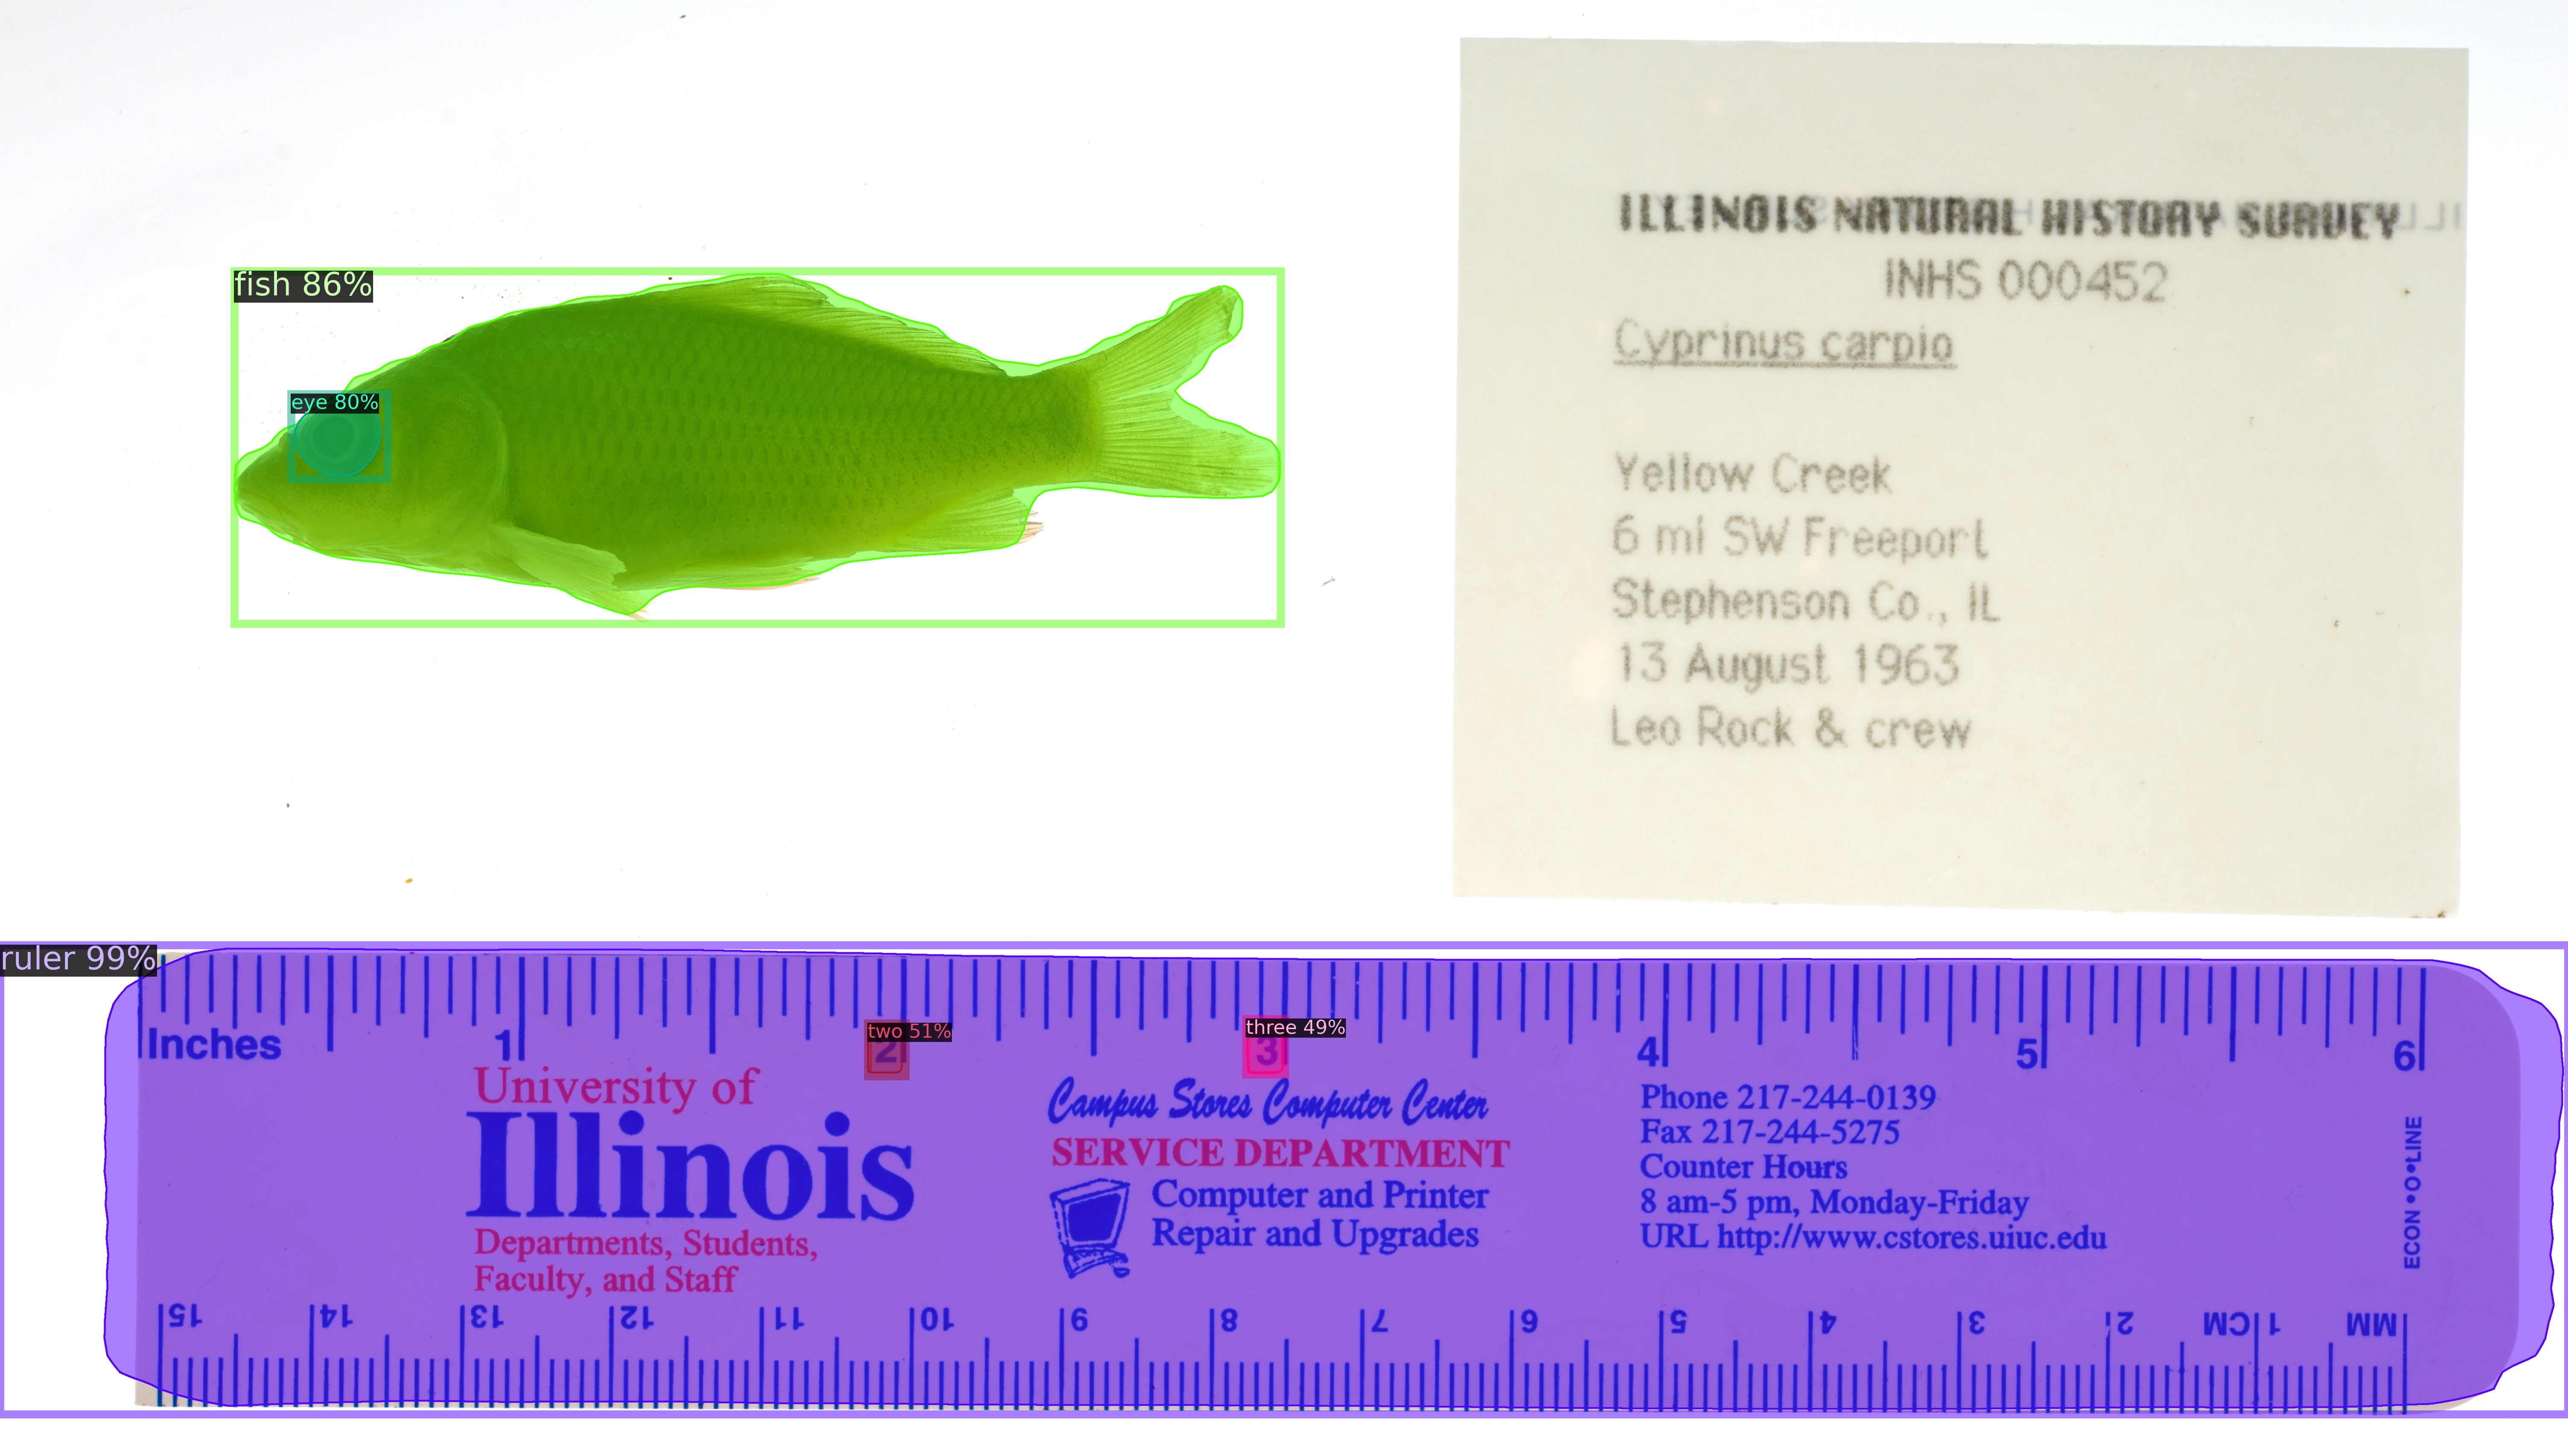
\includegraphics[width=.45\textwidth]{images/teaser1_crop}
  \hspace{4mm}
  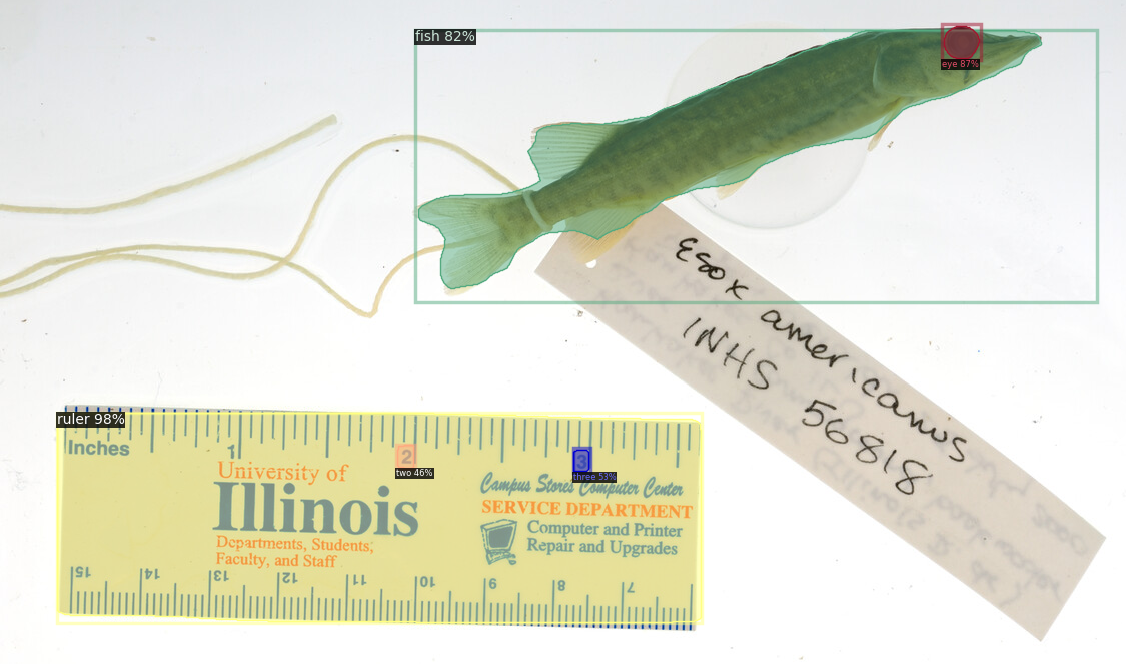
\includegraphics[width=.45\textwidth]{images/teaser2_crop}
  \caption{Initial object detection on specimen images using Detectron2~\cite{wu2019detectron2}}
  \Description{Fish predictions}
  \label{fig:teaser}
\end{teaserfigure}

%%
%% This command processes the author and affiliation and title
%% information and builds the first part of the formatted document.
\maketitle

\section{Introduction}

\todo{Sentences I didn't use: Over the last few decades, cyberinfrastructure development, advances in digitization, and the open science tenor, have helped support global access to natural history. OR
Global access to natural history collections has accelerated over the last few decades to advances in cyberinfrastructure, digitization, and the general open science tenor}

Over the last several decades advances in computing, imaging, and
cyberinfrastructure have supported the growth of digital natural history collections. In the U.S., programs, such as the National Science Foundation’s former Advancing Digitization of Biodiversity Collections (ADBC) program, which ran for
nearly a decade, and the current Infrastructure Capacity for Biological Research program have supported the digital acquisition and dissemination of data and images for millions of biological specimens. These resources are globally available through a wide range of open access repositories, enabling researchers, educators, students, and the general public to examine and compare in ways previously unimaginable. Significant challenges surface, however, when researchers seek to apply computational methods to these data items,
due to both image quality and metadata issues.
% (As researchers seek to apply computational methods, and explore AI, significant challenges surface..) 

Unfortunately, potential scientific advances are hindered by image quality
problems and the lack of accurate and pertinent metadata
associated with the image collections.
Poor quality images, e.g. with low contrast, inadequate lighting,
out-of-focus or cluttered visual arrangements, provide inadequate input
for automated
image analysis and machine learning algorithms and lead to inferior
computational results.
In order to perform quantitative morphometric analysis of the specimens,
the physical scale of the images (pixels/inch) is needed; thus
requiring the ability to identify and measure rulers in the images.
Many specimen collections do include Darwin Core metadata, detailing
specimen taxon, geographic location, and several other descriptive aspects.
Additionally, some digitization efforts record technical metadata, detailing imaging specifications. While these types of metadata are helpful for a
human examining several images at a time, they are insufficient for researchers seeking to apply computational methods to examine thousands of images
to determine if, for instance, a specific fish grows to different lengths
in different habitats.

Since the digital collections may each contain tens of thousands of images, producing metadata for each image via a manual process is prohibitively labor-intensive and infeasible. Methods for automatically computing metadata from images are therefore needed to fully exploit biological image repositories for scientific discovery.
As a step towards improving metadata in specimen research image collections, members of Drexel University's Metadata Research Center are developing methods to automatically analyze fish images and
extract a set of data features that provide important metadata about the
digitized specimen.
The research is being conducted as part of the Biology Guided Neural Networks (BGNN) project, which aims to develop a novel class of artificial neural networks that exploit machine readable and predictive knowledge associated with specimen images, phylogenies and anatomy ontologies.
Using a combination of machine learning and image informatics tools and techniques, we can accurately determine general image quality and metadata, such as fish quantity and location within images, fish orientation, and
image scaling based on ruler identification and measurement. Image scaling
allows us to compute quantitative features about the fish specimens, such
as their length and area.  In order to test and validate our methods, they
were  applied to a set of 7,247
images drawn from the Illinois Natural History Survey (INHS) Collection.
The following section of the paper provides contextual background for this work, followed by the research goals and objectives, and a review of our research methods. Next, the results are presented, followed by a discussion. The conclusion highlights key findings and identifies next steps.

\section{Related Work}
\textbf{Todo}
\subsection{Metadata for Image Collection}
\todo{Wasn't looking for a citation but stumbled upon this paper: \url{https://journals.plos.org/plosone/article?id=10.1371/journal.pone.0207636}, might be worth a skim}
Metadata development is intertwined with the development of digital technology. A wide range of metadata standards are applicable to metadata supporting image description as well as technical aspects, and have been used in a range of image repositories. Examples of Descriptive schemes include X, y, z... Examples of technical schemes include... The use varies across communities, and application technique is primarily manual. Research evaluating such schemes XXX, show XXX. 

Natural history collections generally use a sub-set of such standards. Darwin Core, a globally adopted standard overseen by the Taxonomic Data Working Group (TDWG).  [Jane continue here on some of this, and then with preservation/image quality less]

Fish species dataset in Pakistan Shah 2019 \cite{Shah2019FishPakFS},

\subsection{Metadata generation?}

\subsection{Fish Image Analysis}

Image analysis has been utilized to examine and process images of fish
for well over two decades \cite{Zion2000InvivoFS,Saberioon2017ApplicationOM}. It is an important
application of technology both for marine science, in the study of aquatic
species, habitats and ecosystems, and for the seafood industry, in the
development of automated fish sorting and grading systems, as well as
fisheries management. Many of these computational analyses focus on
the recognition and classification 
of the fish present in an image.  The computational methods employed for
fish image analysis have followed the general trends in the AI field.
Hu et al.~\cite{HuJing2012Fscb} presented a method of classifying species
of fish based on color and texture features and a multi-class support
vector machine (MSVM) \cite{Vapnik1999AOS}.
Li and Hong \cite{Li2014IdentificationOF} computed eleven shape and color
features from fish images that were distilled down to four, using Principal
Component Analysis, and derived a linear model
that could discriminate between four different fishes.
%  Kinda unimpressive. Let's leave out.
% Saitoh \cite{Saitoh2015ImagebasedFR}
% utilized a Random Forest method \cite{Breiman2001RF} on manually-derived
% geometric, Bag of visual words (BoVW) and color features 
Rodrigues et al.~\cite{RodriguesMarcoT.A2015Ecda} explored several
combinations of features extraction, input classifiers and clustering
algorithms to produce a method that could distinguish between 10 different
types of fish with a 92\% accuracy.
%  Again, not too impressive. Let's leave out.
% Ogunlana 2015 \cite{Ogunlana2015FCU},
% In this paper, a Support Vector Machine (SVM)-based technique for the elimination of the limitations of some existing techniques and improved classification of fish species is proposed. The technique is based on the shape features of fish that was divided into two subsets with the first comprising 76 fish as training set while the second comprises of 74 fish as testing set. The body and the five fin lengths; namely anal, caudal, dorsal, pelvic and pectoral were extracted in centimeter (cm). Results based on the new technique show a classification accuracy of 78.59%, which is significantly higher than what obtained for ANN, KNN and K-mean clustering-based algorithms.
Salman et al.~\cite{Salman2016FishSC} employed a deep Convolution Neural
Networks (CNN) \cite{LeCun2004LMG} together with classification based on
K-Nearest Neighbor and Support Vector Machines trained on the features
extracted by the CNN. They achieved 90\%
accuracy when identifying 15 different fish in challenging underwater
digital images.
% Unimpressive. Do not include.
% Sung 2017 \cite{Sung2017VisionBR},
% Underwater vision has specific characteristics such as high attenuation of lights, severe noise and haze in the images. For real-time fish detection using underwater vision, this paper proposes convolutional neural network based techniques based on You Only Look Once algorithm. Actual fish video images were used to evaluate the reliability and accuracy of the proposed method. As a result, the network recorded 93% classification accuracy, 0.634 intersection over union between predicted bounding box and ground truth, and 16.7 frames per second of fish detection. It also outperforms another fish detector using sliding window algorithm and classifier trained with histogram of oriented gradient features and support vector machine.
% Not digging it.
% Hasija 2017 \cite{Hasija2017FishSC},
% This paper proposes a novel method based on an improved image-set matching approach, which makes use of Graph-Embedding Discriminant Analysis. In contrast to the state-of-the-art methods, which operate on single input images, our method makes, use of explicit image set matching which renders it robust computationally.
% Not this one either
% Sayed 2018 \cite{SayedGehadIsmail2018AAFS},
% This paper proposed an automated fish species identification system based on a modified crow search optimization algorithm. Median filtering is applied for image smoothing and removing noise through reducing the variation of intensities between the neighbors. Then, a k-mean clustering algorithm is used to segment the fish image into multiple segments. Shape-based and texture-based feature extraction process for classification is presented. A new modified binary version of crow search algorithm is proposed to reduce the data dimensionality of the extracted features. Finally, support vector machine and decision trees are implemented for classification and the fish species are classified based on either their class including Actinopterygii and Chondrichthyes or based on their order. Total of 270 images with different species, classes and orders are used for evaluation of the proposed system. The experimental results show that the proposed system achieves the highest classification accuracy compared to state-of-the-art algorithms. Also, the results show that the overall fish species identification system obtains on average of 10 folds, 96% classification accuracy for classification based on class and 74% for classification based on fish order.
Utilizing texture, anchor points, and statistical measurements,
Alsmadi et al.~\cite{Alsmadi2019RFE} implemented fish
classification through a meta-heuristic algorithm known as Memetic Algorithm (Genetic Algorithm with Simulated Annealing) with back-propagation algorithm (MA-B Classifier). They were able to classify 24 fish families with 90\%
accuracy.
% Nope
% Sharmin 2019 \cite{Sharmin2019MVB},
% the new generation people of Bangladesh lacks the knowledge of local freshwater fish. For this problem, a solution has been found with the collaboration of vision-based technology. As a solution, a machine-vision based local freshwater fish recognition system is presented that can be proceed with an image of fish captured with a mobile or handheld device and recognize the fish in order to introduce the fish. To demonstrate the utility of the proposed expert system, several experiments are performed. At first, a set of fourteen features, which consists of four types of features, are presented. Then the color image has been converted into gray-scale image and the gray-scale histogram is formed. Image segmentation takes place using histogram-based method and then the features are extracted. PCA is used for decreasing the feature numbers. Three classifiers are used for recognizing fish, where SVM gives the highest accuracy showing a value of 94.2%.
%  I want to see the paper before I cite it.
% Banan 2020 \cite{Banan2020DeepLA}
% Hence, in this study, a deep learning neural network as a smart, real-time and non-destructive method was developed and applied to automate the identification of four economically important carp species namely common carp (Cyprinus carpio), grass carp (Ctenopharingodon idella), bighead carp (Hypophtalmichthys nobilis) and silver carp (Hypophthalmichthys molitrix). The obtained results proved that our approach, evaluated through 5-fold cross-validation, achieved the highest possible accuracy of 100 %. The achieved high level of classification accuracy was due to the ability of the suggested deep model to build a hierarchy of self-learned features, which was in accordance with the hierarchy of these fish’s identification keys. In conclusion, the proposed convolutional neural network (CNN)-based method has a single and generic trained architecture with promising performance for fish species identification.
Iqbal et al.~\cite{Iqbal2021AutomaticFS} used a modified
AlexNet \cite{AlexNet2012} model to classify six different fish species
with 90\% accuracy.
% In this paper, we presented an automated system for identification and classification of fish species. It helps the marine biologists to have greater understanding of the fish species and their habitats. The proposed model is based on deep convolutional neural networks. It uses a reduced version of AlexNet model comprises of four convolutional layers and two fully connected layers. A comparison is presented against the other deep learning models such as AlexNet and VGGNet. The four parameters are considered that is number of convolu- tional layers and number of fully-connected layers, number of iterations to achieve 100% accuracy on training data, batch size and dropout layer. The results show that the proposed and modified AlexNet model with less number of layers has achieved the testing accuracy of 90.48% while the original AlexNet model achieved 86.65% over the untrained bench- mark fish dataset. The inclusion of dropout layer has enhanced the overall performance of our proposed model. It contain less training images, less memory and it is also less compu- tational complex.
%  No paper. No reference
% Xu 2021 \cite{Xu2021TransferLA},
% Scientific studies on species identification in fish have considerable significance in aquatic ecosystems and quality evaluation. The morphological differences between different fish species are obvious. Machine learning methods use artificial prior knowledge to extract fish features, which is time-consuming, laborious, and subjective. Recently, deep learning-based identification of fish species has been widely used. However, fish species identification still faces many challenges due to the small scale of fish samples and the imbalance of the number of categories. For example, the model is prone to being overfitted, and the performance of the classifier is biased to the fish species of most samples. To solve the above problems, this paper proposes a fish species identification approach based on SE-ResNet152 and class-balanced focal loss. First, visualization analysis and image preprocessing of fish datasets are carried out. Second, the SE-ResNet152 model is constructed as a generalized feature extractor and is migrated to the target dataset. Finally, we apply the class-balanced focal loss function to train the SE-ResNet152 model, and realize fish species identification on three fish image views (body, head, and scale). The proposed method was tested on the Fish-Pak public dataset and achieved 98.80%, 96.67%, and 91.25% accuracy on the three fish image views, respectively. To ensure the superior performance of the proposed method, we performed an experimental comparison with other methods involving SENet154, DenseNet121, ResNet18, ResNet152, VGG16, cross-entropy, and focal loss. Comprehensive empirical analyses reveal that the proposed method achieves good performance on the three fish image views and outperforms common methods.


% \textbf{Orientation, Length, Size, Weight and Shape}\newline
Especially in industrial settings it is necessary to automatically
detect the orientation, length and weight of fish during handling
and processing.
In some instances it is necessary to computationally straighten the
fish in the images \cite{MuozBenavent2018EnhancedFB} before further
processing can be attempted.
Balaban et al.~\cite{Balaban2010UsingIA} demonstrated that image analysis
and data fitting may be used to predict the weight of salmons with high
accuracy.
% After harvesting , salmon is sorted by species, size, and quality. This is generally manually done by op-erators. Automation would bring repeatability, objectivity, and record-keeping capabilities to these tasks. Machinevision (MV) and image analysis have been used in sorting many agricultural products. Four salmon species weretested: pink (Oncorhynchus gorbuscha), red (Oncorhynchus nerka), silver (Oncorhynchus kisutch), and chum (On-corhynchus keta). A total of 60 whole fish from each species were first weighed, then placed in a light box to taketheir picture. Weight compared with view area as well as length and width correlations were developed. In additionthe effect of “hump” development (see text) of pink salmon on this correlation was investigated. It was possible topredict the weight of a salmon by view area, regardless of species, and regardless of the development of a humpfor pinks. Within pink salmon there was a small but insignificant difference between predictive equations for theweight of “regular” fish and “humpy” fish. Machine vision can accurately predict the weight of whole salmon forsorting.
% Konovalov 2017 \cite{KonovalovD2017RDfA},
% Fast and low cost image collection and processing is often required in aquaculture farms for quality/size attributes and breeding programs. For example, the absolute physical dimensions of fish (in millimeters or inches) could be estimated from electronic images. The absolute scale of the photographed fish is often unknown or requires additional hardware, data- collection and/or management overheads. One cost and time effective solution is to capture the absolute scale (in pixels-per- millimeter or dots-per-inch) by including a measuring ruler in the photographed scene. To assist that type of workflow, we designed a relatively simple image-processing algorithm that automatically located a sufficiently large section of the ruler in a given image. The algorithm utilized the Fast Fourier Transform and was designed to be free from adjustable parameters and therefore did not require training or calibration. The algorithm was tested on 445 images of Barramundi (Asian sea bass, Lates calcarifer), where a millimeter-graded ruler was included in each image. The algorithm achieved precision of 98% (on the original, 10, 20, 70, 80 90 degree rotated images) and 95-96% on 40, 50, 60 degree rotated images. \newline
% Konovalov 2018 \cite{Konovalov2018AutomaticSO},
% In aquaculture breeding programs where large numbers of fish need to be rapidly phenotyped, the absolute physical dimensions of fish (in millimeters or inches) are often required to be extracted from electronic images in order to measure the size of the fish. While it is possible to infer the length of the fish in pixels, the absolute scale of the image (in pixels-per-millimeter or dots-per- inch) is largely unknown without a reference grid, or requires additional hardware, data collection and/or record-keeping management overheads. One cost and time effective solution is to capture the absolute scale by including a measuring ruler in the photographed scene and from which a computer program can automatically identify the scale of the photo and calculate fish morphometric measurements. To assist such workflow, this study developed an algorithm that automatically detects a ruler in a given image, and automatically extracts its scale as distance (in fractional number of pixels) betw. The algorithm was applied to 445 publicly available images of barramundi or Asian seabass (Lates calcarifer), where a millimeter-graded ruler was included in each image. Convolutional Neural Network (CNN) was trained to segment the images into ruler, background, fish and label sections. Then the distance-extraction algorithm was applied to the ruler section of the images. The false-negative rate was less than 2%, where the ruler graduation distances could not be extracted in only 2-6 (out of 445) images even when the test images were rotated up to 90 degrees. The mean absolute relative error (MARE) of the inferred distances was 1-2%.\newline
Konovalov et al.~\cite{Konovalov2019AutomaticWE} presented a method for
accurate automatic weight estimation of fish using a Convolutional Neural
Network (CNN), data fitting, and a ruler detection/measurement
method \cite{Konovalov2018AutomaticSO}.
% Approximately 2,500 weights and corresponding images of harvested Lates calcarifer (Asian seabass or barra- mundi) were collected at three different locations in Queensland, Australia. Two instances of the LinkNet-34 segmentation Convo- lutional Neural Network (CNN) were trained. The first one was trained on 200 manually segmented fish masks with excluded fins and tails. The second was trained on 100 whole-fish masks. The two CNNs were applied to the rest of the images and yielded automatically segmented masks. The one-factor and two-factor simple mathematical weight-from-area models were fitted on 1072 area-weight pairs from the first two locations, where area values were extracted from the automatically segmented masks. When applied to 1,400 test images (from the third location), the one- factor whole-fish mask model achieved the best mean absolute percentage error (MAPE), MAPE = 4.36%. Direct weight-from- image regression CNNs were also trained, where the no-fins based CNN performed best on the test images with MAPE = 4.28%.
Hao et al.~\cite{Hao2015TheMO} provide an excellent review of fish
measurement efforts that utilize machine vision.
% This study reviewed the methods of fish size measurement through machine vision. Length and area are important information that can help fishers manage fish scientifically and conveniently. This information could be used to calculate the volume and weight according to their relation; other information could also be calculated. Machine vision is more effective, economical and faster than traditional methods.
Azarmdel et al.~\cite{Azarmdel2019DevelopingAO} developed a system
capable of determining the orientation of a trout and segmenting its fins,
which are used as cutting points, with an accuracy over 99\%.
% Fish processing in small and medium fish supplying centers requires an intelligent system to operate on different sizes. Therefore, an image processing algorithm was developed to extract the proper head and belly cutting points according to the trout dimensions. The algorithm detects the fish orientation and location of pectoral, anal, pelvic, and caudal fins. In this study, each of the trout images was divided into slices along its length in order to segment the fins and extract cutting points. The channel ‘B’ of RGB color space was considered in both initial segmentation and fin detection stages among the examined channels of RGB, HSV, and L*a*b* color spaces. The back-belly and head-tail sides were detected with an accuracy of 100% based on gray intensity values and head to tail ratio, respectively. Furthermore, performing an analysis of variance (ANOVA) resulted in an F-value of 64.82 among the fins. Conducting a t-test among the mean intensity values of the fins and non-fin regions of channel ‘B’ resulted in the highest distinction with t-values of 90.30, 78.07, 74.28, and 86.01 with p < 0.01 for the pectoral, pelvic, anal, and caudal fins paired with the corresponding non-fin region, respectively. The results showed that the selected ‘B’ channel is the adequate one for fin segmentation. The fin detection process showed an overall sensitivity, specificity, and accuracy of 86.05%, 99.97%, and 99.87%, respectively. By solving the line determination error in 8.24% and the extra object error in 4.12% of the samples, the overall fin identification accuracy was 100%. Finally, after extracting the fin regions, the start point of the pectoral fin and the end point of the anal fin will be applied in the trout processing system as the head and belly cutting points, respectively.

Another application of image analysis to fish images is the evaluation
fish freshness, a computation usually performed on the color features of
the images.
Tappi et al.~\cite{Tappi2017ComputerVS} assess the freshness of frozen
fish by computing a change of color and an eye concavity index.
% The evaluation of fish freshness can be per- formed using chemical, sensory and physical methods. Besides sensory methods, several instrumental techniques have been applied with the objective of replacing sensory assessment. The aim of this study was to set up and test objective physical methods mainly based on computer vision system (CVS) to assess red mullet (Mullus barba- tus) freshness evolution during 10 days of storage, at two different storage temperatures (0 and 4 °C). To check the effectiveness of the purposed physical methods, CVS fea- tures (loss in the epidermis pigmentation, development of gill mucus and eye concavity index) and firmness have been compared with chemical trimethylamine content and sensory (QIM) attribute scores. As expected, fish degrada- tion was faster at the higher temperature. Instrumental tex- ture evaluation of fish by penetration test enabled to detect distinctive firmness changes due to onset and resolution of rigor mortis, and the successive tenderization phenomenon. Among CVS parameters, the epidermis pigmentation loss, and particularly the eye shape modification (eye concavity index) evidenced a high sensibility for the estimation of fresh red mullet quality loss, as a function of the two differ- ent storage conditions, and a good agreement with trimeth- ylamine content and QIM response evolution.
Taheri-Garavand et al.~\cite{TaheriGaravand2019RealtimeNM} diagnosed the 
freshness of common carp during ice storage. They utilize color feature
extraction and Artificial Neural Networks (ANN) to place fish in four
freshness categories with 93\% accuracy.
% In the current research, the potential of a novel method based on the artificial neural network was investigated to diagnose the freshness of common carp (Cyprinus carpio) during ice storage. Fish as an aquaculture product has high nutrients and low-fat content. So, people have consumed it as a safe and high-value foodstuff in their daily diet. Investigation of fish freshness is proposed as a significant issue in the aquaculture industry since fish spoils rapidly. The applied system of this study is comprised of the following steps: First, images of samples were captured and the pre-processing operation was done on the images. Then, particular channels including R, G, B, H, S, I, L*, a*, and b* were computed. Next, feature extraction was performed to obtain 6 types of texture features from each channel. Afterward, the hybrid Artificial Bee Colony-Artificial Neural Network (ABC-ANN) algorithm was applied to select the best features. Finally, the Support Vector Machine (SVM), K-Nearest Neighbor (K-NN) and Artificial Neural Network (ANN) algorithms as the most common methods were used to classify fish images. The best performance of the K-NN classifier was calculated in the k = 8 neighborhood size with the accuracy of 90.48. The best kernel function for the SVM algorithm was polynomial with C, sigma, and accuracy of 1, 2 and 91.52 percent, respectively. In this system, the input layer has consisted of 22 neurons based on the feature selection operation and 4 classes including most fresh, fresh, fairly fresh and spoiled have been used as the number of output layer. At the end, the best results of the MLP networks were achieved by LM learning algorithm and 6 neurons in the hidden layer with the 22–10–4 topology and accuracy of 93.01 percent.
% The achieved results demonstrate the high performance of the ANN classifier for evaluation of common carp freshness during ice storage as a rapid, accurate, non-destructive, real-time and automated method. It shows the potential of computer vision method in combination with artificial neural networks as an intelligent technique for evaluation of fish freshness.
A similar approach was developed by Lalabadi et al.~\cite{Lalabadi2020FishFC}.
% Developing new techniques to determine fish freshness and quality can enhance nutritional value of the overall household food basket. In this research, digital image analysis was utilized to assess the freshness of rainbow trout fish by tracing the color attributes of its eyes and gills. The image data were collected from left and right eyes and gills in a 10-day ice-storage duration, and color components were extracted in RGB, HSV, and L*a*b* color spaces. Analysis of variance revealed that the RGB components of both eyes and gills had a significant change towards getting brighter during the ice-storage. Feature extraction was fulfilled from the color spaces, and then artificial neural networks (ANNs) and support vector machines (SVMs) were applied for classification of the ice-storage durations. The overall accuracies of the developed models demonstrated that the ANN somewhat outperformed the SVM for both the extracted features from the eyes and gills. Moreover, the gills’ features could describe the variance in the storage durations more efficiently than those extracted from the eyes. Finally, it was concluded that the applied colorimetric system along with the developing models could be employed as a successful non-destructive approach for evaluation of fish freshness.


\begin{comment}
\textbf{Not Used}\newline
(Kinda vague. More about food, then fish, G{\"u}m{\"u} 2011 \cite{Gm2011MachineVA}),
(In Turkish, Iscimen 2014 \cite{Iscimen2014ImageAM},
Iscimen 2015 \cite{Iscimen2015ClassificationOF}),
(Not based on images (sonar?) Kinjo 2014 \cite{KinjoAtsushi2014Scoi}),
(Too basic, Wang 2015 \cite{Huihui2015StudyOT}),
(Not so interesting, a very engineered, constrained imaging set up, Miranda 2017 \cite{MIRANDA201741}),

(A review of all types of sensing systems for quality checkin, Bernardo 2020 \cite{Bernardo2020FishQI}),
(Another review, but in Trends in Analytical Chemistry. I think we can 
skip it. Not so technical, Dowlati 2012 \cite{Dowlati2012ApplicationOM}),

(Simple industrial system. Computing length, Sung 2020 \cite{Sung2020AutomaticGF}),

(These are 3D. Don't want to go there, Bock 2018 \cite{BockAlexander2018TITE},
Williams 2020 \cite{Williams:2020:UIF})

(A review that is not quite focused enough, Petrov 2020 \cite{Petrov2020Overview}),
(Don't have access to it, and I have a newer review, Zion 2012 \cite{Zion2012ReviewTU}),
\end{comment}



\section{Goals and Objectives}

Digitized specimen collections offer numerous outstanding opportunities
for new scientific studies and discoveries.

The amount of data is immense, with image collections containing 10,000's
of entries. These discoveries will only be possible
with computational techniques that can process this vast amount of data.

These image-based computational techniques are hampered by both poor
image quality and the lack of high-quality and pertinent metadata
associated with collections.

For example, a study may require images that contain only one fish with a
given level of lighting and contrast. Additionally, performing quantitative
investiations into the morphology of the specimens requires knowing
the physical scale of the images, i.e.~pixels/inch.

Given the many thousands of images that have and will be acquired of
biological specimens, it is infeasible to generate the needed metadata
via manual, i.e. via human input, methods.  It is critical to deploy
computational techniques that will automate the process of generating
the metatdata that is essential for downstream analyses and studies.

In order to address the need for fish specimen image metadata that can
support scientific investigations we have begun the deployment of
both off-the-shelf and custom-written software that automatically
generates a variety of metadata from a publicly-available biological
image repository.  The types of metadata being produced are related
to image quality, content and scale, and should provide the information
necessary for advanced quantitative studies of the digitized specimens.

The automated metadata generation methods for our project were developed
to work on a specific set of images, the INHS\ Fish
Collection~\cite{INHS}.  Most of these images have been configured,
produced and acquired with a standard procedure.  The images used for
our study contain one fish placed on a bright, white background and
contain an information tag and the same ruler.  See 
Figure \ref{fig:teaser} for two example images from the collection.
While training and focusing our system on images with very similar
compositions and visual properties may limit its immediate applicability,
our efforts do demonstrate the potential that machine learning and
image informatics techniques have for automatically generating metadata
for biological specimen image collections.


\section{Methods}
Our process for metadata generation can be broken into three steps: object detection with Facebook's Detectron2 machine learning library (subsequently referred to as \verb|detectron|), image informatics analysis at the pixel level, and calculations on the results of the previous steps to determine higher level metadata properties.
% \todo{Definitely need to explain somewhere in more detail about our current admissibility criteria for images. Not sure where I want to put it yet so just leaving it as a todo}

\subsection{Detectron}
A prerequisite task to performing any advanced metadata property generation
is finding the specimens (and other relevant objects) within the collection
images. Object detection has been a broadly active field of study in recent
years \cite{zou2019object}, and has resulted in a number of well-tested, purpose-built architectures. We elected to use Facebook AI Research's \verb|detectron| tool \cite{wu2019detectron2}, and specifically its implementation of the Mask R-CNN architecture \cite{he2018mask}, for object detection in our project.
\verb|detectron| is built on \verb|pytorch|~\cite{NEURIPS2019_9015} and provides a relatively straightforward method for training on COCO~\cite{DBLP:journals/corr/LinMBHPRDZ14} format datasets. It is able to handle an arbitrary number of object classes, and can classify an arbitrary number of object within a given image. For our project, we are currently using it to identify five object classes: fish, fish eyes, rulers, and the numbers 2 and 3 on rulers.

\begin{wraptable}{r}{5.5cm}
    \centering
      \caption{Training dataset}
    \label{tab:dataset}
    \begin{tabular}{cc}
        \toprule
        \textbf{Class} & \textbf{Number of Instances}\\
        \midrule
        Fish & 297\\
        Ruler & 1496\\
        Eye & 456\\
        Two & 100\\
        Three & 100\\
      \bottomrule
    \end{tabular}
\end{wraptable}

Table \ref{tab:dataset} lists the number of instances for each class 
used in our training dataset.
All of the training data was labeled by hand using \verb|makesense.ai| \cite{make-sense}
% While the ultimate goal of the project is to generalize to images from a variety of specimen collections, we have thus far focused only
on images from the INHS\ Fish Collection \cite{INHS}.
Using \verb|detectron|'s default training scheme, the model was trained for \(100,000\) epochs. All instance types were included in a single object detection model. The total loss\todo{Find and specify which loss function was used} began at \(2.948\) and ended at \(0.158\) for the training data.

\begin{comment}
\begin{verbatim}
|  category  | #instances   |  category  | #instances   |  category  | #instances   |
|:----------:|:-------------|:----------:|:-------------|:----------:|:-------------|
|    fish    | 297          |   ruler    | 1496         |    eye     | 456          |
|    two     | 100          |   three    | 100          |            |              |
|   total    | 2449         |            |              |            |              |

Iterations: 100,000

Initial: {"data_time": 0.004866079999999329, "fast_rcnn/cls_accuracy": 0.115234375,
"fast_rcnn/false_negative": 0.1686291000841043,
"fast_rcnn/fg_cls_accuracy": 0.2782012195121951, "iteration": 5, "loss_box_reg": 0.40475407242774963,
"loss_cls": 1.8559419512748718, "loss_mask": 0.6982034742832184, "loss_rpn_cls": 0.05218731239438057,
"loss_rpn_loc": 0.007734265644103289, "lr": 0.00011990000000000001, "mask_rcnn/accuracy": 0.2920252418802887,
"mask_rcnn/false_negative": 0.9506743610216735, "mask_rcnn/false_positive": 0.2467277275646746,
"roi_head/num_bg_samples": 115.0, "roi_head/num_fg_samples": 13.0, "rpn/num_neg_anchors": 251.25,
"rpn/num_pos_anchors": 4.75, "time": 0.2812129614999961, "total_loss": 2.9480794025585055}

Final: {"data_time": 0.006645713496254757, "eta_seconds": 0.0, "fast_rcnn/cls_accuracy": 0.984375,
"fast_rcnn/false_negative": 0.0, "fast_rcnn/fg_cls_accuracy": 1.0, "iteration": 99999,
"loss_box_reg": 0.054501257836818695, "loss_cls": 0.03908616118133068, "loss_mask": 0.06379510834813118,
"loss_rpn_cls": 0.0010549294238444418, "loss_rpn_loc": 0.005114196799695492, "lr": 0.02,
"mask_rcnn/accuracy": 0.9722937165937804, "mask_rcnn/false_negative": 0.012800597698663846,
"mask_rcnn/false_positive": 0.05609636495338312, "roi_head/num_bg_samples": 115.75,
"roi_head/num_fg_samples": 12.25, "rpn/num_neg_anchors": 246.5, "rpn/num_pos_anchors": 9.5,
"time": 0.3563086399990425, "total_loss": 0.15775199318886735}
\end{verbatim}
\end{comment}
\subsection{Pixel Analysis}
The masks and bounding boxes produced by \verb|detectron| are generally quite good, although they almost never completely or tightly enclose the
detected objects.
This is problematic for the detected fish objects in our analyzed images,
where the most accurate segmentation is desired.
The mask may include additional background as part of the fish, or the
bounding box may clip away part(s) of the fish. To solve these
shortcomings, we utilize pixel analysis methods commonly found in image
informatics to produce more accurate objects masks and bounding boxes.

\subsubsection{Threshold Adjustment}
The first calculation in the pixel analysis process determines the cutoff intensity between what constitutes the foreground (i.e.~the fish) and background of the image.
Initially, the calculation is based on the bounding box and mask generated by
\verb|detectron|. Specimen images are read in as gray scale, and pixels in the image are treated as unsigned integers between 0 and 255.
Otsu thresholding, a technique that maximizes the variance between the 
foreground and background intensities, is used to compute an initial cutoff value between foreground and background. 
While the Otsu value occasionally generates an accurate mask as is, usually
the contrast between foreground and background is low and much of the lighter parts of the fish (such as its tail fin) are marked as background.

To overcome this under-segmentation, the threshold value should be
either adjusted up or down, depending on if the background is lighter or darker than the fish.
For our current dataset, the background is always lighter (i.e.~closer to 255), so the threshold value needs to be scaled up to include more of the
foreground image.
% Precisely how much to scale this value by is difficult to determine.
For optimal results the scaling should be dependent on the
contrast between the background and foreground,
which can be affected by
% both how washed out the image is and
the level of pigmentation of the fish.
% To take this into account, we compute the mean intensity of the foreground and background pixels, then use these intensity values and the difference between them to scale the threshold value.
% Even with these values in hand it is not entirely clear how to scale the threshold.
We found that an improved threshold value can be computed as the halfway
point between the Otsu threshold value and the
mean of the background intensities.
This adjusted threshold value
% by 50\% of the difference between the mean of the background and the original threshold value, which 
captures most of fish's fins in most cases, without also masking parts of the background.

\subsubsection{Consolidating the Foreground}
While thresholding has the potential to generate better masks than a neural network (when provided an initial approximate bounding box), it also introduces considerable noise. Single or small groups of errant pixels can be marked as foreground depending on the consistency of the background, and interior pixels of the fish (especially around the fins) can be marked as background. To be useful for generating an accurate bounding box and for subsequent computational analysis, the mask must consist of one single ``blob'' over the fish the contains no holes, and no other pixels disconnected from this blob can be marked as foreground.

To accomplish this, we apply an iterative process of flood filling from all the foreground pixels in the image until a blob is generated that is large enough to constitute the fish. This is another metaparameter, but greater than 10\% of the current bounding box has masked the specimen in all observed cases. Once the fish's blob is found, noise then needs removed. This is done by flood filling from each of the corner of the bounding box where the specimen is not present (all four corners in the overwhelming majority of cases), then taking the inverse of the result. The fish mask is excluded from these corner flood fills, so this process removes all noise from both the background and foreground of the image leaving only a close mask over the fish itself.

\subsubsection{Adjusting the Bounding Box}
With an accurate mask generated, it is then necessary to check whether the bounding box needs expanded or shrunk along any edges. Expansion is done first, buy checking whether any edge intersects with any of the foreground mask pixels. If one does, it is expanded out by 1 pixel. If any edges are expanded, the whole the process, masking and expansion process is repeated to account for any changes in average intensities. Once no edges contain foreground pixels, the mask is the shrunk. This process is more efficient as all that is required is to shrink each edge by one up until the point they contain one or more foreground pixels. Once the shrinkage step is accomplished, the final mask and bounding box have been generated.

\subsubsection{Fallback} The pixel analysis process occasionally fails. This can occur if certain flood fill operations behave unexpectedly, or if the image is too washed out or otherwise atypical for the thresholding process to work correctly. In the event this happens, the original mask and bounding box generated by \verb|detectron| is used for metadata generation.
\subsection{Metadata Generation}
Including what has already been discussed, the following metadata properties are being currently being generated:

\begin{table}[t]
    \centering
    \caption{Metadata properties}
    \label{tab:properties}
    \begin{tabular}{cccp{0.5\linewidth}}
        \toprule
        \textbf{Property} & \textbf{Association} & \textbf{Type} & \textbf{Explanation}\\
        \midrule
        \verb|has_fish| & Overall Image & Boolean & Whether a fish was found in the image.\\
        \verb|fish_count| & Overall Image & Integer & The quantity of fish present.\\
        \verb|has_ruler| & Overall Image & Boolean & Whether a ruler was found in the image.\\
        \verb|ruler_bbox| & Overall Image & 4 Tuple & The bounding box of the ruler (if found).\\
        \verb|scale| & Overall Image & Float & The scale of the image in \(\frac{\mathrm{pixels}}{\mathrm{cm}}\).\\
        \verb|bbox| & Per Fish & 4 Tuple & The top left and bottom right coordinates of what define the bounding box for a fish.\\
        \verb|background.mean| & Per Fish & Float & The mean intensity of the background within a given fish's bounding box.\\
        \verb|background.std| & Per Fish & Float & The standard deviation of the background within a given fish's bounding box.\\
        \verb|foreground.mean| & Per Fish & Float & The mean intensity of the foreground within a given fish's bounding box.\\
        \verb|foreground.std| & Per Fish & Float & The standard deviation of the foreground within a given fish's bounding box.\\
        \verb|centroid| & Per Fish & 4 Tuple & The centroid of a given fish's bitmask.\\
        \verb|primary_axis| & Per Fish & 2D Vector & The unit length primary axis (eigenvector) for the bitmask of a given fish.\\
        \verb|clock_value| & Per Fish & Integer & A fish's primary axis converted into an integer ``clock value'' between 1 and 12.\\
        \verb|length| & Per Fish & Float & The length of a fish in \(\frac{\mathrm{pixels}}{\mathrm{cm}}\).\\
        \verb|mask| & Per Fish & 2D Matrix & The bitmask of a fish in 0's and 1's.\\
        \verb|pixel_analysis_failed| & Per Fish & Boolean & Whether the pixel analysis process failed for a given fish. If \verb|true|, \verb|detectron|'s mask and bounding box were used for metadata generation.\\
        \verb|score| & Per Fish & Float & The percent confidence score output by \verb|detectron| for a given fish.\\
        \verb|has_eye| & Per Fish & Boolean & Whether an eye was found for a given fish.\\
        \verb|eye_center| & Per Fish & 2 Tuple & The centroid of a fish's eye.\\
        \verb|side| & Per Fish & String & The side (i.e.\ \verb|'left'| or \verb|'right'|) of the fish that is facing the camera (dependent on finding its eye).\\
      \bottomrule
\end{tabular}
\end{table}

\verb|has_fish|, \verb|fish_count|, \verb|has_ruler|, \verb|ruler_bbox|, \verb|background.*|, \verb|foreground.*|, \verb|bbox|, \verb|mask|, \verb|score|, and \verb|has_eye| have already been discussed. The remaining properties are determined as follows:
\subsubsection{centroid and eye\_center}
Centroids are provided for masks/bounding boxes generated by \verb|detectron|, and since we do not recalculate the mask of fish eyes we can use that value directly for \verb|eye_center|.

Since we recalculate the mask of the fish, we must recalculate its centroid as well. This can be done via
\begin{equation}
    (\bar{x}, \bar{y}) = (\mathrm{round}(\frac{M_{10}}{M_{00}}), \mathrm{round}(\frac{M_{01}}{M_{00}}))
\end{equation}
where \(M_{00}\) is the pixel area of the fish's blob, \(M_{10}\) is the sum of all the \(x\) values of blob pixels, and \(M_{01}\) is the sum of all the \(y\) values of blob pixels.
\subsubsection{side}
Determining which \verb|side| of the fish is visible is predicated on finding its eye. If an eye is found, the sign of the \(x\) component of the vector from the centroid of the fish to the centroid of the eye specifies which side is up: negative for left and positive for right. This assumes the fish was photographed vertically, which is essentially always the case for all image collections our group has worked on.
\subsubsection{primary\_axis and clock\_value}
The \verb|primary_axis| of a fish can be calculated by taking the covariance\todo{I could explain this in more detail if necessary} of its blob in \(x\) and \(y\), which yields its principle eigenvector. This can be directly assigned to the property. If an eye is present, we specify this axis in the direction of the eye in relation to the fish's centroid.

Our team encoded this information as a ``clock value'' between 1 and 12 when recording it by hand. To convert \verb|principal_axis| to \verb|clock_value|, the sign of \(x\) and \(y\) on the principal axis are used to determine which Cartesian quadrant the fish is angles into relative to its centroid. Depending on this quadrant, we then dot product the principal axis with either \([-1,0]\), \([0,-1]\), \([1,0]\) or \([0,1]\) which correspond to 9, 6, 3 and ``0'' o'clock respectively. The resulting radian value is then converted to a polar displacement in clock value space, and added to the comparative clock value used in the dot product. This then gives the fish's clock value from 0 to \(11.\overline{9}\). Before recording as \verb|clock_value| in the output, the value is rounded to the nearest integer, and in the event of a 0 final result it is replaced with 12.
\subsubsection{scale and length}
\(\frac{\mathrm{pixels}}{\mathrm{inch}}\) can be calculated by measuring the distance between the digits 2 and 3 found on the ruler by \verb|detectron|. Converting this to \(\frac{\mathrm{pixels}}{\mathrm{cm}}\) gives the \verb|scale| metadata property as reported in the output.

For the fish \verb|length| property, it is necessary to determine the furthest points from the centroid of the fish in each direction. Since fish are normally measured in a straight line from their snout down the middle of their trunk, we project every pixel onto the major axis of the fish (as a line through its centroid) before checking the distance. This projection is done by intersecting the line through the point along the tangent of the principal axis and the aforementioned centroid--principal axis line. After checking every pixel, measuring the distance between the two furthest projected points gives the length of the fish in pixels. Multiplying this by \verb|scale| gives the fish \verb|length| in centimeters.
\begin{comment}
\subsection{Consideration}
Just gonna throw some caveats in here, might be its own section might not
\begin{itemize}
    \item Program falls back to using detectron mask and bbox for metadata generation in the event the mask generation/pixel analysis fails. Failure is defined as never finding a cohesive flood filled mask that covers more than 10\% of the detectron bbox initially. Can provide a statistic on how often this occurs.
\end{itemize}
\end{comment}
\section{Results}
Technicians employed by our team have manually generated the 22 metadata properties deemed crucial to the overall BGNN project~\cite{Leipzig2021.01.28.428644} for a large number of INHS images. \(20,699\) total entries were created by 13 technicians that spanned \(8,398\) unique images. Of these \(8,398\) images, \(7,244\) were both not part of the \verb|detectron| training set and meet our current admissibility criteria for what \verb|detectron| and the pixel analysis process can reliably handle. We ran the metadata extraction program on these \(7,244\) images.

Our automated process currently generates 7 of the 22 core metadata properties: \verb|if_fish| (\verb|has_fish|), \verb|fish_number| (\verb|fish_count|), \verb|if_ruler| (\verb|has_ruler|), \verb|specimen_angled| (\verb|clock_value|), \verb|specimen_view| (\verb|side|), \verb|brightness| (derived from \verb|background.mean| and \verb|foreground.mean|), and \verb|if_background_uniform| (\verb|background.std|). In addition, our process also calculates bounding boxes and fish lengths in centimeters.\todo{Talk more about what we can and can't verify and how.}

\subsection{Fish Detection}
All images in the INHS dataset contain exactly one fish. For \(7,209\) of the specimen images, one fish was detected. For 25 of the images, 2 fish were detected, 3 fish were detected for 3 images, and for 7 images no fish were found. In the case of greater than 1 fish, 9 of the 28 contained tags which overlapped the fish and were themselves labeled as a second fish. Of the remaining 17, \verb|detectron| erroneously labeled the fish as two separate fish objects, or labeled a subsection of the fish a second time.

\subsection{Ruler Detection}
For all but 2 of the \(7,244\) images \verb|detectron| was able to find the ruler.\todo{Not sure if I can phrase it that way or not since I haven't looked at all the images to see if the ruler itself was found or something else was labeled a ruler} For an additional 56 images, the ruler itself was found but the ``2'' and/or the ``3'' on it was not, so a scale calculation could not be performed.

\subsection{Side Detection}
For 246 of the images \verb|detectron| was unable to find a fish eye. Of the remaining \(6,998\) images where it did, the correct side (\verb|left| or \verb|right|) was detected in all but 6 cases.

\subsection{Clock Value}
Clock position values were successfully generated for \(6,991\) of the images. Of those, all but 8 were within \(\pm{}1\) of the correct result.

\subsection{Brightness/Uniformity Results?}
\textbf{Todo}: I can try to do this but I need to set up the infrastructure, we probably need to discuss a plan of action for this.

\subsection{Mask and Bounding Box}
\begin{figure}[H]
  \centering
  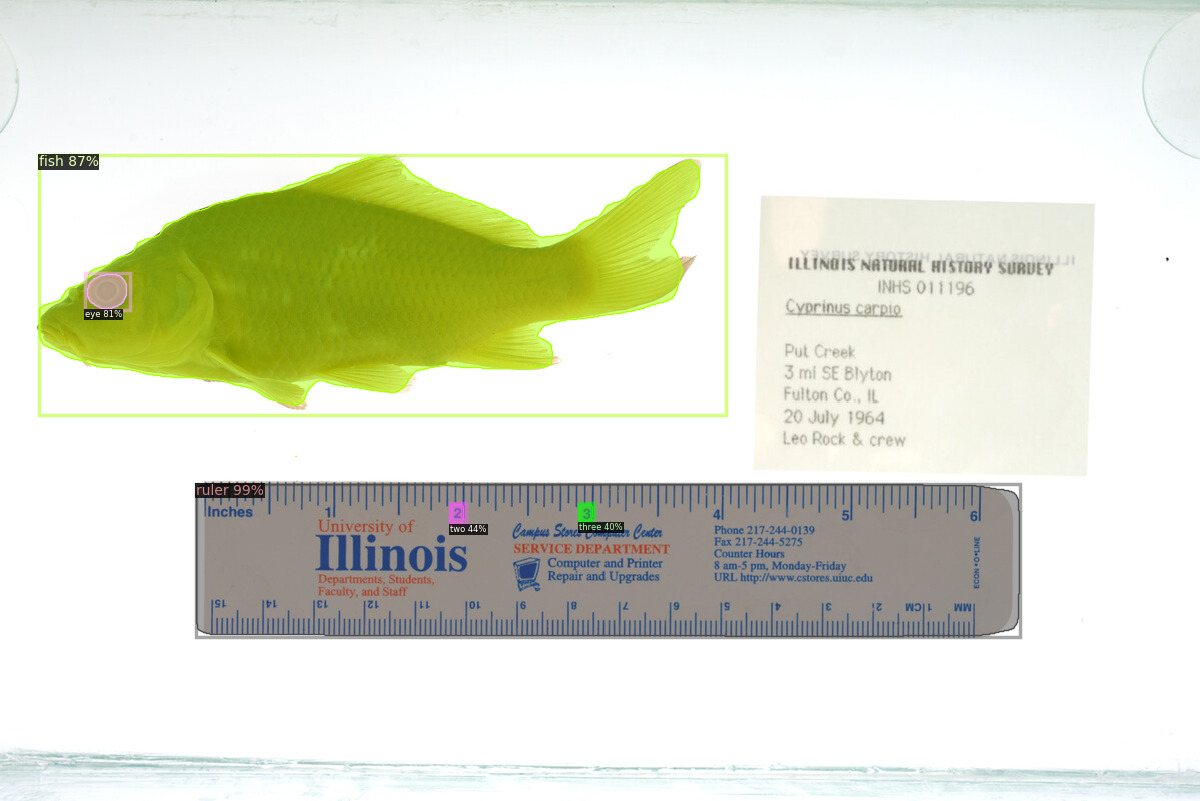
\includegraphics[width=0.49\linewidth]{images/011196_pred}
  
\includegraphics[width=0.49\linewidth]{images/011196_mask}
  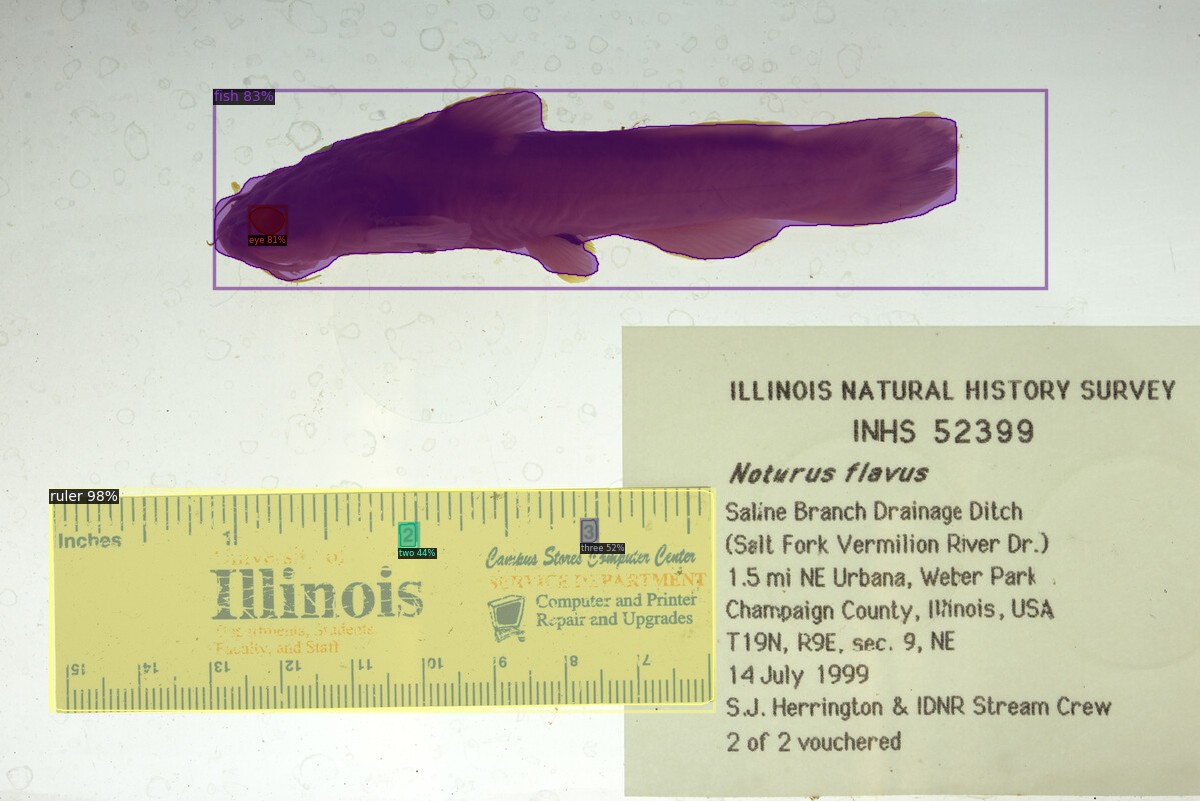
\includegraphics[width=0.49\linewidth]{images/52399_pred}
  
\includegraphics[width=0.49\linewidth]{images/52399_mask}
  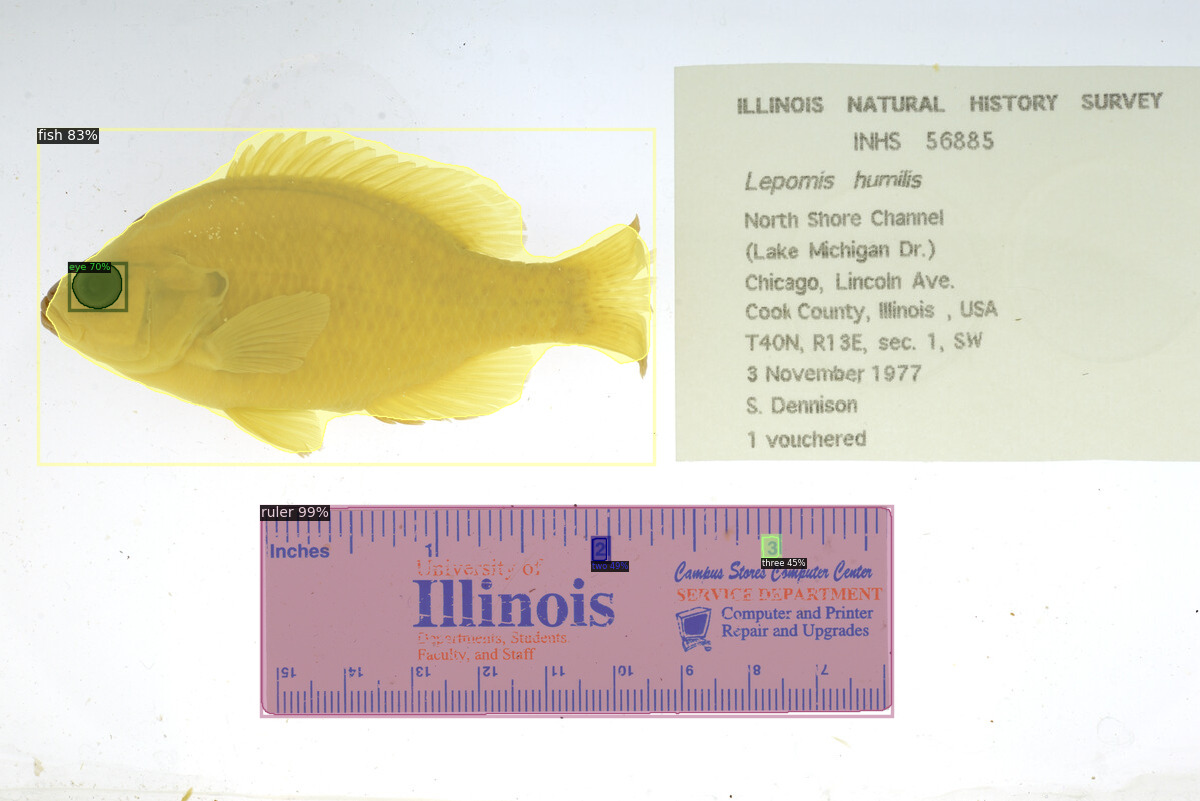
\includegraphics[width=0.49\linewidth]{images/56885_pred}
  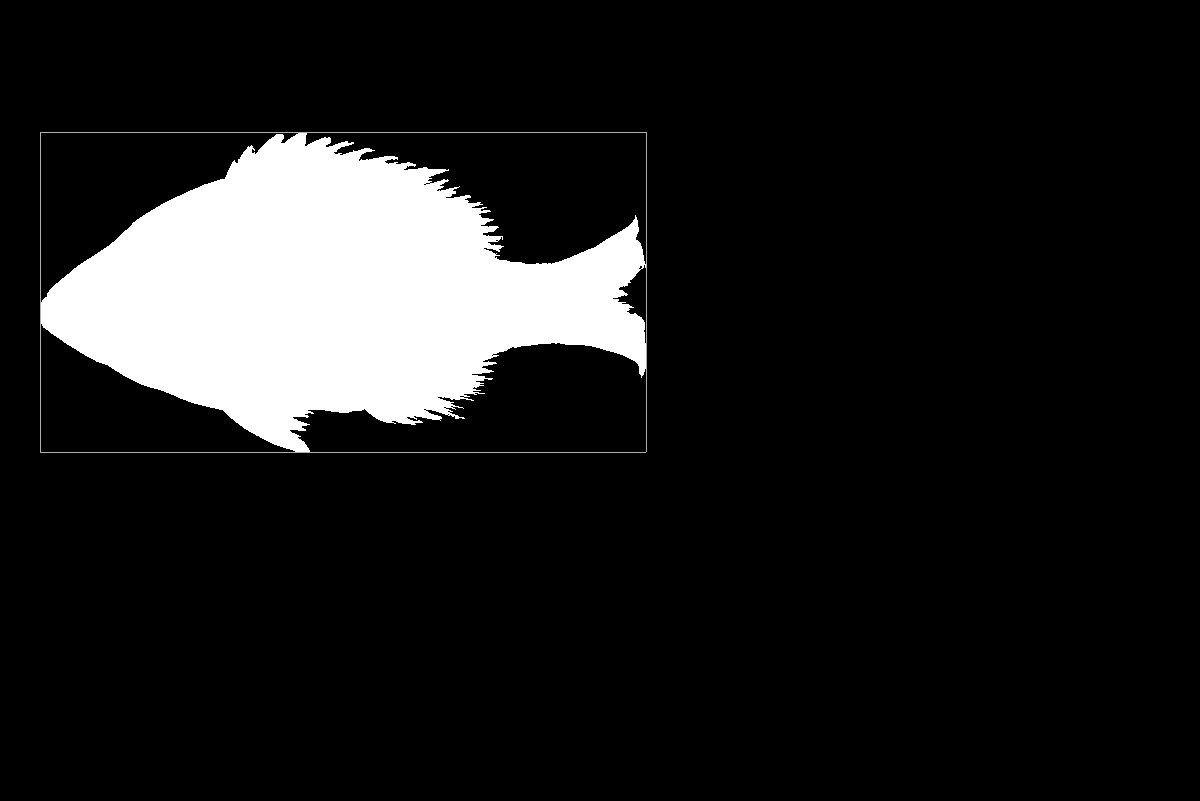
\includegraphics[width=0.49\linewidth]{images/56885_mask}
  \caption{Examples of masks and bounding boxes from detectron (left) and pixel analysis (right).}
  \Description{Bounding box and mask examples}
\end{figure}
Fish bounding boxes were calculated for all \(7,237\) images in which a fish was found. All but 263 of these were generated via pixel analysis, with those 263 falling back to the original \verb|detectron| bounding box. \textbf{Todo}: Anything more than this is going to need hand checked.

\subsection{Length}
Fish lengths were calculated for \(7,179\) of the images. \textbf{Todo}: Anything more than this is going to need hand checked.
\begin{comment}
\begin{verbatim}
What I think should be the final results:

Right: 6956
Errored: 0
No eye: 246
No fish: 10
Wrong wrong: 35
Total: 7247
Percent right: 0.959845453291017
Percent right that didn't error: 0.9949935631526248

-----------------------

Pixel analysis failed: 0.036336004421110804

-----------------------

My hand checking of the ''wrong wrong'' fish:
               My guess, Yasin spreadsheet
INHS_FISH_101109.jpg: 9, 11, I'm wrong although it's fairly curved
INHS_FISH_56818.jpg: 4, 2, I'm wrong although there's a tag that is likely messing things up
INHS_FISH_57607.jpg: 3, 9, I'm wrong
INHS_FISH_57001.jpg: 4, 2, I'm wrong although there's a tag that is likely messing things up
INHS_FISH_63953.jpg: 3, 9, I'm wrong
INHS_FISH_51100.jpg: 3, 9, I'm wrong
INHS_FISH_80528.jpg: 3, 8, I'm wrong
INHS_FISH_6370.jpg: 3, 9, I'm wrong
INHS_FISH_54157.jpg: 9, 7, I'm arguably wrong although it's very curved
INHS_FISH_80987.jpg: 9, 3, I'm wrong although this one is a fairly atypical image

INHS_FISH_58647.jpg: 9, 7, I'm right
INHS_FISH_8415.jpg: 9, 6, I'm right
INHS_FISH_5041.jpg: 9, 11, very curved averages to about 9
INHS_FISH_52821.jpg: 9, 7, I'm arguably right although the fish is damaged and its head points to ~7
INHS_FISH_6696.jpg: 9, 7, I'm right
INHS_FISH_75252.jpg: 9, 6, I'm right
INHS_FISH_79498.jpg: 9, 6, I'm right
INHS_FISH_45744.jpg: 9, 5, I'm right
INHS_FISH_47579.jpg: 9, 6, I'm right
INHS_FISH_64599.jpg: 9, 6, I'm right
INHS_FISH_74550.jpg: 9, 5, I'm right
INHS_FISH_101664.jpg: 9, 6, I'm right
INHS_FISH_100861.jpg: 9, 6, I'm right
INHS_FISH_60589.jpg: 3, 9, I'm right
INHS_FISH_53469.jpg: 9, 1, I'm right
INHS_FISH_44694.jpg: 9, 6, I'm right
INHS_FISH_54921.jpg: 9, 6, I'm right
INHS_FISH_44645.jpg: 10, 8, I'm right
INHS_FISH_50459.jpg: 9, 11, I'm right although the fish is damaged and its head points to ~11
INHS_FISH_68061.jpg: 9, 6, I'm right
INHS_FISH_74716.jpg: 9, 6, I'm right
INHS_FISH_80976.jpg: 9, 6, I'm right
INHS_FISH_57977.jpg: 9, 6, I'm right
INHS_FISH_45377.jpg: 9, 6, I'm right
INHS_FISH_47142.jpg: 9, 6, I'm right

Verdict: For only 10 of the 35 am I actually wrong and all of those are either curved, atypical
images with tags, or something on the wrong side was detected as an eye (so the clock value is backwards).

\end{verbatim}
\end{comment}

\section{Discussion}
\textbf{Todo}: Will need some sort of intro/framing paragraph
\subsection{Results}\todo{Just going to put the results discussion in small sections and we can change it later if that doesn't make sense}
\subsubsection{Object Detection}
\begin{figure}[H]
  \centering
  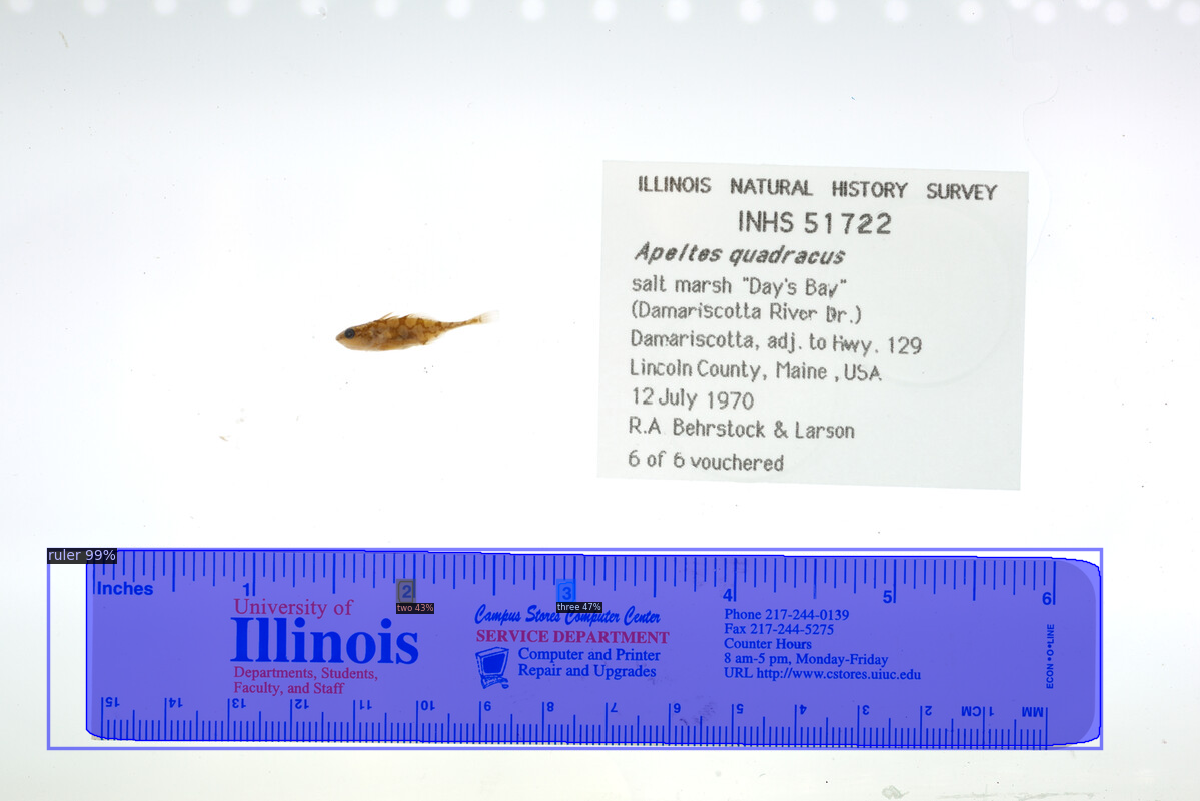
\includegraphics[width=0.49\linewidth]{images/none1}
  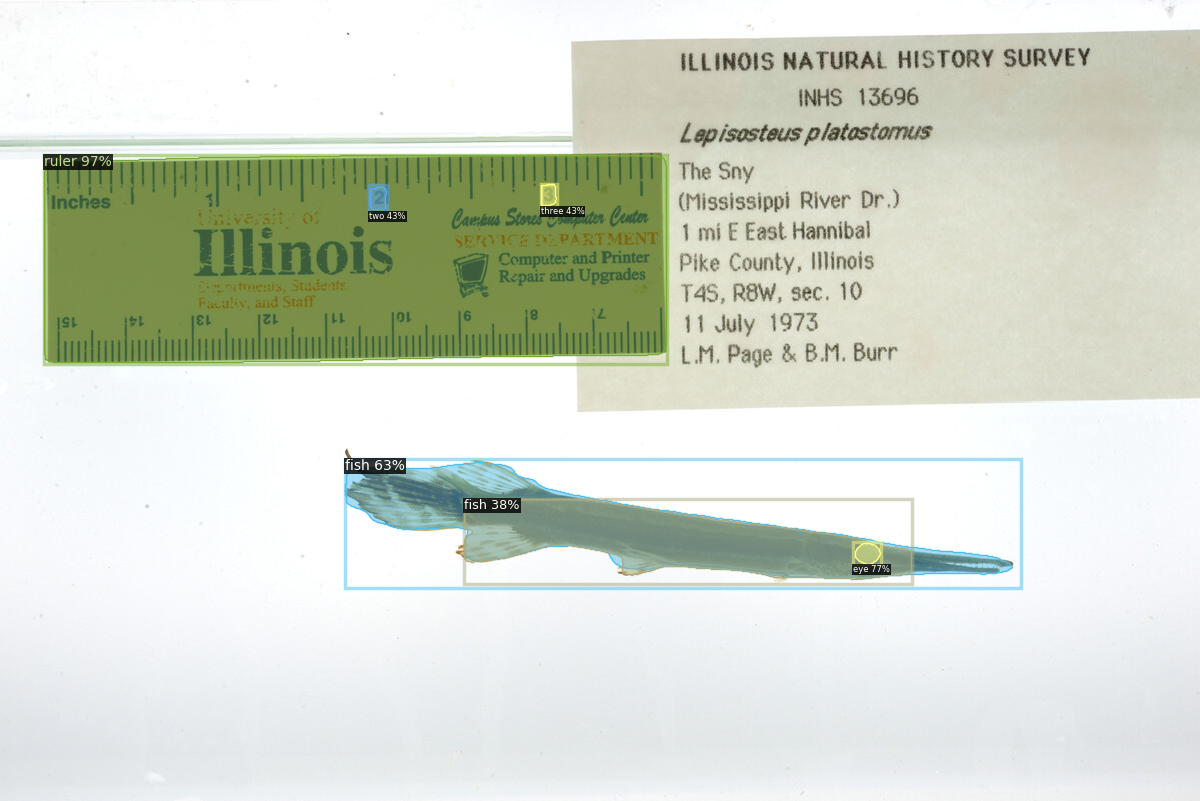
\includegraphics[width=0.49\linewidth]{images/double1}
  \caption{An example of a fish that was not detected (left) and a fish that was detected twice (right).}
  \Description{Mislabeled eye on a catfish}
\end{figure}

\begin{itemize}
    \item Worked fairly well all things considered
    \item Talk about which fish failed
    \item Talk about which rulers failed
\end{itemize}
\subsubsection{Side Detection}
\begin{figure}[H]
  \centering
  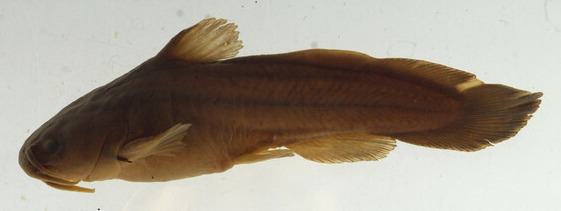
\includegraphics[width=0.49\linewidth]{images/wrong_side_orig}
  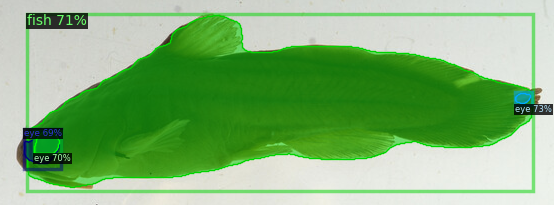
\includegraphics[width=0.49\linewidth]{images/wrong_side1}
  \caption{A fish for which a splotch on its tail fin was labeled the most likely eye.}
  \Description{Mislabeled eye on a catfish}
\end{figure}
For all 6 of the cases where an eye was detected but the \verb|side| value was wrong, a spot on the wrong side of the fish was labeled as the most likely eye within the bounding box of the fish. There were an additional 17 images for which the automated process generated a result that did not match the manually created data. For these remaining cases the manual data was incorrect, giving the automated system an error rate \(2.8\) times lower than than the human error rate.

\subsubsection{Clock Value}
\begin{figure}[H]
  \centering
  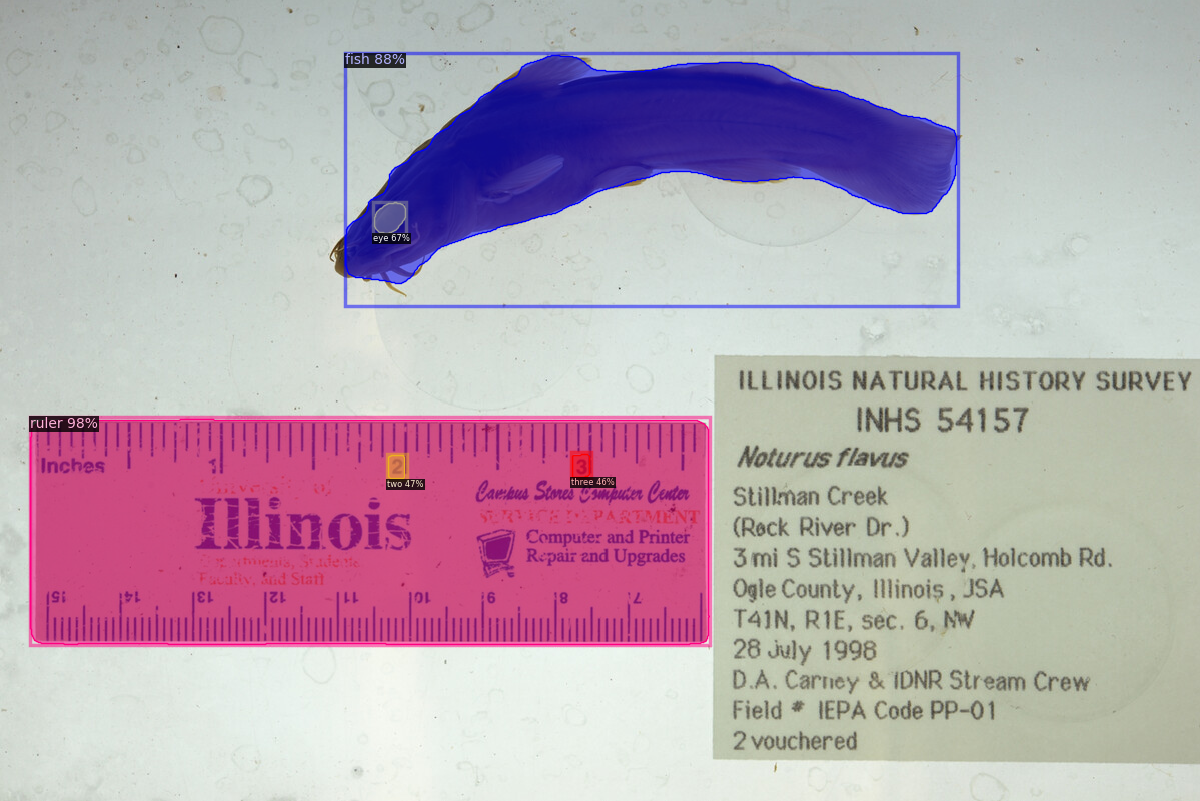
\includegraphics[width=0.49\linewidth]{images/curved1}
  %\includegraphics[width=0.49\linewidth]{images/}
  \caption{An example of a heavily curved specimen.}
  \Description{Mislabeled eye on a catfish}
\end{figure}
Of the specimens for which clock values were generated, 33 did not match the manually created data (within a tolerance of \(\pm{}1\)).For 25 of those the human generated data was incorrect, giving the automated process a \(3.1\) times lower error rate. Of the remaining 8, 2 specimens were quite curved making it difficult to assign a clear angle value. The other 6 were values of 3 instead of 9 or vice versa that resulted from a mislabeled eye as discussed in the previous section. A small number of images (such as on the right in Figure~\ref{fig:teaser}) have tags that overlap with the fish. These tags were light enough that they were correctly labeled as background by the pixel analysis.

\subsubsection{Mask and Bounding Box}

\subsubsection{Brightness?}

\subsubsection{Length}

\subsection{Future Work}
\begin{itemize}
    \item Further fine tuning of pixel analysis (e.g.\ thresholding on different regions of the bbox).
    \item Generalizing ruler reading.
    \item Training on a progressively larger number of image collections to hopefully gain reasonable generality for the whole class of fish specimen images.
    \item Adding things like seahorses and eels.
    \item Fitting a ``spine'' to specimen.
\end{itemize}
\section{Conclusion}
\textbf{Todo}

\bibliographystyle{ACM-Reference-Format}
\bibliography{paper}

%\begin{figure}[H]
%  \centering
%  \includegraphics[width=\linewidth]{images/}
%  \caption{}
%  \Description{}
%\end{figure}

\begin{comment}
\pagebreak{}
\section{Introduction}~\label{demo-intro}
ACM's consolidated article template, introduced in 2017, provides a
consistent \LaTeX\ style for use across ACM publications, and
incorporates accessibility and metadata-extraction functionality
necessary for future Digital Library endeavors. Numerous ACM and
SIG-specific \LaTeX\ templates have been examined, and their unique
features incorporated into this single new template.

If you are new to publishing with ACM, this document is a valuable
guide to the process of preparing your work for publication. If you
have published with ACM before, this document provides insight and
instruction into more recent changes to the article template.

The ``\verb|acmart|'' document class can be used to prepare articles
for any ACM publication --- conference or journal, and for any stage
of publication, from review to final ``camera-ready'' copy, to the
author's own version, with {\itshape very} few changes to the source.

\section{Template Overview}
As noted in the introduction, the ``\verb|acmart|'' document class can
be used to prepare many different kinds of documentation --- a
double-blind initial submission of a full-length technical paper, a
two-page SIGGRAPH Emerging Technologies abstract, a ``camera-ready''
journal article, a SIGCHI Extended Abstract, and more --- all by
selecting the appropriate {\itshape template style} and {\itshape
  template parameters}.

This document will explain the major features of the document
class. For further information, the {\itshape \LaTeX\ User's Guide} is
available from
\url{https://www.acm.org/publications/proceedings-template}.

\subsection{Template Styles}

The primary parameter given to the ``\verb|acmart|'' document class is
the {\itshape template style} which corresponds to the kind of publication
or SIG publishing the work. This parameter is enclosed in square
brackets and is a part of the {\verb|documentclass|} command:
\begin{verbatim}
  \documentclass[STYLE]{acmart}
\end{verbatim}

Journals use one of three template styles. All but three ACM journals
use the {\verb|acmsmall|} template style:
\begin{itemize}
\item {\verb|acmsmall|}: The default journal template style.
\item {\verb|acmlarge|}: Used by JOCCH and TAP.
\item {\verb|acmtog|}: Used by TOG.
\end{itemize}

The majority of conference proceedings documentation will use the {\verb|acmconf|} template style.
\begin{itemize}
\item {\verb|acmconf|}: The default proceedings template style.
\item{\verb|sigchi|}: Used for SIGCHI conference articles.
\item{\verb|sigchi-a|}: Used for SIGCHI ``Extended Abstract'' articles.
\item{\verb|sigplan|}: Used for SIGPLAN conference articles.
\end{itemize}

\subsection{Template Parameters}

In addition to specifying the {\itshape template style} to be used in
formatting your work, there are a number of {\itshape template parameters}
which modify some part of the applied template style. A complete list
of these parameters can be found in the {\itshape \LaTeX\ User's Guide.}

Frequently-used parameters, or combinations of parameters, include:
\begin{itemize}
\item {\verb|anonymous,review|}: Suitable for a ``double-blind''
  conference submission. Anonymizes the work and includes line
  numbers. Use with the \verb|\acmSubmissionID| command to print the
  submission's unique ID on each page of the work.
\item{\verb|authorversion|}: Produces a version of the work suitable
  for posting by the author.
\item{\verb|screen|}: Produces colored hyperlinks.
\end{itemize}

This document uses the following string as the first command in the
source file:
\begin{verbatim}
\documentclass[acmsmall]{acmart}
\end{verbatim}

\section{Modifications}

Modifying the template --- including but not limited to: adjusting
margins, typeface sizes, line spacing, paragraph and list definitions,
and the use of the \verb|\vspace| command to manually adjust the
vertical spacing between elements of your work --- is not allowed.

{\bfseries Your document will be returned to you for revision if
  modifications are discovered.}

\section{Typefaces}

The ``\verb|acmart|'' document class requires the use of the
``Libertine'' typeface family. Your \TeX\ installation should include
this set of packages. Please do not substitute other typefaces. The
``\verb|lmodern|'' and ``\verb|ltimes|'' packages should not be used,
as they will override the built-in typeface families.

\section{Title Information}

The title of your work should use capital letters appropriately -
\url{https://capitalizemytitle.com/} has useful rules for
capitalization. Use the {\verb|title|} command to define the title of
your work. If your work has a subtitle, define it with the
{\verb|subtitle|} command.  Do not insert line breaks in your title.

If your title is lengthy, you must define a short version to be used
in the page headers, to prevent overlapping text. The \verb|title|
command has a ``short title'' parameter:
\begin{verbatim}
  \title[short title]{full title}
\end{verbatim}

\section{Authors and Affiliations}

Each author must be defined separately for accurate metadata
identification. Multiple authors may share one affiliation. Authors'
names should not be abbreviated; use full first names wherever
possible. Include authors' e-mail addresses whenever possible.

Grouping authors' names or e-mail addresses, or providing an ``e-mail
alias,'' as shown below, is not acceptable:
\begin{verbatim}
  \author{Brooke Aster, David Mehldau}
  \email{dave,judy,steve@university.edu}
  \email{firstname.lastname@phillips.org}
\end{verbatim}

The \verb|authornote| and \verb|authornotemark| commands allow a note
to apply to multiple authors --- for example, if the first two authors
of an article contributed equally to the work.

If your author list is lengthy, you must define a shortened version of
the list of authors to be used in the page headers, to prevent
overlapping text. The following command should be placed just after
the last \verb|\author{}| definition:
\begin{verbatim}
  \renewcommand{\shortauthors}{McCartney, et al.}
\end{verbatim}
Omitting this command will force the use of a concatenated list of all
of the authors' names, which may result in overlapping text in the
page headers.

The article template's documentation, available at
\url{https://www.acm.org/publications/proceedings-template}, has a
complete explanation of these commands and tips for their effective
use.

Note that authors' addresses are mandatory for journal articles.

\section{Rights Information}

Authors of any work published by ACM will need to complete a rights
form. Depending on the kind of work, and the rights management choice
made by the author, this may be copyright transfer, permission,
license, or an OA (open access) agreement.

Regardless of the rights management choice, the author will receive a
copy of the completed rights form once it has been submitted. This
form contains \LaTeX\ commands that must be copied into the source
document. When the document source is compiled, these commands and
their parameters add formatted text to several areas of the final
document:
\begin{itemize}
\item the ``ACM Reference Format'' text on the first page.
\item the ``rights management'' text on the first page.
\item the conference information in the page header(s).
\end{itemize}

Rights information is unique to the work; if you are preparing several
works for an event, make sure to use the correct set of commands with
each of the works.

The ACM Reference Format text is required for all articles over one
page in length, and is optional for one-page articles (abstracts).

\section{CCS Concepts and User-Defined Keywords}

Two elements of the ``acmart'' document class provide powerful
taxonomic tools for you to help readers find your work in an online
search.

The ACM Computing Classification System ---
\url{https://www.acm.org/publications/class-2012} --- is a set of
classifiers and concepts that describe the computing
discipline. Authors can select entries from this classification
system, via \url{https://dl.acm.org/ccs/ccs.cfm}, and generate the
commands to be included in the \LaTeX\ source.

User-defined keywords are a comma-separated list of words and phrases
of the authors' choosing, providing a more flexible way of describing
the research being presented.

CCS concepts and user-defined keywords are required for for all
articles over two pages in length, and are optional for one- and
two-page articles (or abstracts).

\section{Sectioning Commands}

Your work should use standard \LaTeX\ sectioning commands:
\verb|section|, \verb|subsection|, \verb|subsubsection|, and
\verb|paragraph|. They should be numbered; do not remove the numbering
from the commands.

Simulating a sectioning command by setting the first word or words of
a paragraph in boldface or italicized text is {\bfseries not allowed.}

\section{Tables}

The ``\verb|acmart|'' document class includes the ``\verb|booktabs|''
package --- \url{https://ctan.org/pkg/booktabs} --- for preparing
high-quality tables.

Table captions are placed {\itshape above} the table.

Because tables cannot be split across pages, the best placement for
them is typically the top of the page nearest their initial cite.  To
ensure this proper ``floating'' placement of tables, use the
environment \textbf{table} to enclose the table's contents and the
table caption.  The contents of the table itself must go in the
\textbf{tabular} environment, to be aligned properly in rows and
columns, with the desired horizontal and vertical rules.  Again,
detailed instructions on \textbf{tabular} material are found in the
\textit{\LaTeX\ User's Guide}.

Immediately following this sentence is the point at which
Table~\ref{tab:freq} is included in the input file; compare the
placement of the table here with the table in the printed output of
this document.

\begin{table}
  \caption{Frequency of Special Characters}
  \label{tab:freq}
  \begin{tabular}{ccl}
    \toprule
    Non-English or Math&Frequency&Comments\\
    \midrule
    \O & 1 in 1,000& For Swedish names\\
    $\pi$ & 1 in 5& Common in math\\
    \$ & 4 in 5 & Used in business\\
    $\Psi^2_1$ & 1 in 40,000& Unexplained usage\\
  \bottomrule
\end{tabular}
\end{table}

To set a wider table, which takes up the whole width of the page's
live area, use the environment \textbf{table*} to enclose the table's
contents and the table caption.  As with a single-column table, this
wide table will ``float'' to a location deemed more
desirable. Immediately following this sentence is the point at which
Table~\ref{tab:commands} is included in the input file; again, it is
instructive to compare the placement of the table here with the table
in the printed output of this document.

\begin{table*}
  \caption{Some Typical Commands}
  \label{tab:commands}
  \begin{tabular}{ccl}
    \toprule
    Command &A Number & Comments\\
    \midrule
    \texttt{{\char'134}author} & 100& Author \\
    \texttt{{\char'134}table}& 300 & For tables\\
    \texttt{{\char'134}table*}& 400& For wider tables\\
    \bottomrule
  \end{tabular}
\end{table*}

Always use midrule to separate table header rows from data rows, and
use it only for this purpose. This enables assistive technologies to
recognise table headers and support their users in navigating tables
more easily.

\section{Math Equations}
You may want to display math equations in three distinct styles:
inline, numbered or non-numbered display.  Each of the three are
discussed in the next sections.

\subsection{Inline (In-text) Equations}
A formula that appears in the running text is called an inline or
in-text formula.  It is produced by the \textbf{math} environment,
which can be invoked with the usual
\texttt{{\char'134}begin\,\ldots{\char'134}end} construction or with
the short form \texttt{\$\,\ldots\$}. You can use any of the symbols
and structures, from $\alpha$ to $\omega$, available in
\LaTeX~\cite{Lamport:LaTeX}; this section will simply show a few
examples of in-text equations in context. Notice how this equation:
\begin{math}
  \lim_{n\rightarrow \infty}x=0
\end{math},
set here in in-line math style, looks slightly different when
set in display style.  (See next section).

\subsection{Display Equations}
A numbered display equation---one set off by vertical space from the
text and centered horizontally---is produced by the \textbf{equation}
environment. An unnumbered display equation is produced by the
\textbf{displaymath} environment.

Again, in either environment, you can use any of the symbols and
structures available in \LaTeX\@; this section will just give a couple
of examples of display equations in context.  First, consider the
equation, shown as an inline equation above:
\begin{equation}
  \lim_{n\rightarrow \infty}x=0
\end{equation}
Notice how it is formatted somewhat differently in
the \textbf{displaymath}
environment.  Now, we'll enter an unnumbered equation:
\begin{displaymath}
  \sum_{i=0}^{\infty} x + 1
\end{displaymath}
and follow it with another numbered equation:
\begin{equation}
  \sum_{i=0}^{\infty}x_i=\int_{0}^{\pi+2} f
\end{equation}
just to demonstrate \LaTeX's able handling of numbering.

\section{Figures}

The ``\verb|figure|'' environment should be used for figures. One or
more images can be placed within a figure. If your figure contains
third-party material, you must clearly identify it as such, as shown
in the example below.
\begin{figure}[h]
  \centering
  %\includegraphics[width=\linewidth]{sample-franklin}
  \caption{1907 Franklin Model D roadster. Photograph by Harris \&
    Ewing, Inc. [Public domain], via Wikimedia
    Commons. (\url{https://goo.gl/VLCRBB}).}
  \Description{A woman and a girl in white dresses sit in an open car.}
\end{figure}

Your figures should contain a caption which describes the figure to
the reader.

Figure captions are placed {\itshape below} the figure.

Every figure should also have a figure description unless it is purely
decorative. These descriptions convey what’s in the image to someone
who cannot see it. They are also used by search engine crawlers for
indexing images, and when images cannot be loaded.

A figure description must be unformatted plain text less than 2000
characters long (including spaces).  {\bfseries Figure descriptions
  should not repeat the figure caption – their purpose is to capture
  important information that is not already provided in the caption or
  the main text of the paper.} For figures that convey important and
complex new information, a short text description may not be
adequate. More complex alternative descriptions can be placed in an
appendix and referenced in a short figure description. For example,
provide a data table capturing the information in a bar chart, or a
structured list representing a graph.  For additional information
regarding how best to write figure descriptions and why doing this is
so important, please see
\url{https://www.acm.org/publications/taps/describing-figures/}.

\subsection{The ``Teaser Figure''}

A ``teaser figure'' is an image, or set of images in one figure, that
are placed after all author and affiliation information, and before
the body of the article, spanning the page. If you wish to have such a
figure in your article, place the command immediately before the
\verb|\maketitle| command:
\begin{verbatim}
  \begin{teaserfigure}
    \includegraphics[width=\textwidth]{sampleteaser}
    \caption{figure caption}
    \Description{figure description}
  \end{teaserfigure}
\end{verbatim}

\section{Citations and Bibliographies}

The use of \BibTeX\ for the preparation and formatting of one's
references is strongly recommended. Authors' names should be complete
--- use full first names (``Donald E. Knuth'') not initials
(``D. E. Knuth'') --- and the salient identifying features of a
reference should be included: title, year, volume, number, pages,
article DOI, etc.

The bibliography is included in your source document with these two
commands, placed just before the \verb|\end{document}| command:
\begin{verbatim}
  \bibliographystyle{ACM-Reference-Format}
  \bibliography{bibfile}
\end{verbatim}
where ``\verb|bibfile|'' is the name, without the ``\verb|.bib|''
suffix, of the \BibTeX\ file.

Citations and references are numbered by default. A small number of
ACM publications have citations and references formatted in the
``author year'' style; for these exceptions, please include this
command in the {\bfseries preamble} (before the command
``\verb|\begin{document}|'') of your \LaTeX\ source:
\begin{verbatim}
  \citestyle{acmauthoryear}
\end{verbatim}

  Some examples.  A paginated journal article \cite{Abril07}, an
  enumerated journal article \cite{Cohen07}, a reference to an entire
  issue \cite{JCohen96}, a monograph (whole book) \cite{Kosiur01}, a
  monograph/whole book in a series (see 2a in spec. document)
  \cite{Harel79}, a divisible-book such as an anthology or compilation
  \cite{Editor00} followed by the same example, however we only output
  the series if the volume number is given \cite{Editor00a} (so
  Editor00a's series should NOT be present since it has no vol. no.),
  a chapter in a divisible book \cite{Spector90}, a chapter in a
  divisible book in a series \cite{Douglass98}, a multi-volume work as
  book \cite{Knuth97}, a couple of articles in a proceedings (of a
  conference, symposium, workshop for example) (paginated proceedings
  article) \cite{Andler79, Hagerup1993}, a proceedings article with
  all possible elements \cite{Smith10}, an example of an enumerated
  proceedings article \cite{VanGundy07}, an informally published work
  \cite{Harel78}, a couple of preprints \cite{Bornmann2019,
    AnzarootPBM14}, a doctoral dissertation \cite{Clarkson85}, a
  master's thesis: \cite{anisi03}, an online document / world wide web
  resource \cite{Thornburg01, Ablamowicz07, Poker06}, a video game
  (Case 1) \cite{Obama08} and (Case 2) \cite{Novak03} and \cite{Lee05}
  and (Case 3) a patent \cite{JoeScientist001}, work accepted for
  publication \cite{rous08}, 'YYYYb'-test for prolific author
  \cite{SaeediMEJ10} and \cite{SaeediJETC10}. Other cites might
  contain 'duplicate' DOI and URLs (some SIAM articles)
  \cite{Kirschmer:2010:AEI:1958016.1958018}. Boris / Barbara Beeton:
  multi-volume works as books \cite{MR781536} and \cite{MR781537}. A
  couple of citations with DOIs:
  \cite{2004:ITE:1009386.1010128,Kirschmer:2010:AEI:1958016.1958018}. Online
  citations: \cite{TUGInstmem, Thornburg01, CTANacmart}. Artifacts:
  \cite{R} and \cite{UMassCitations}.

\section{Acknowledgments}

Identification of funding sources and other support, and thanks to
individuals and groups that assisted in the research and the
preparation of the work should be included in an acknowledgment
section, which is placed just before the reference section in your
document.

This section has a special environment:
\begin{verbatim}
  \begin{acks}
  ...
  \end{acks}
\end{verbatim}
so that the information contained therein can be more easily collected
during the article metadata extraction phase, and to ensure
consistency in the spelling of the section heading.

Authors should not prepare this section as a numbered or unnumbered {\verb|\section|}; please use the ``{\verb|acks|}'' environment.

\section{Appendices}

If your work needs an appendix, add it before the
``\verb|\end{document}|'' command at the conclusion of your source
document.

Start the appendix with the ``\verb|appendix|'' command:
\begin{verbatim}
  \appendix
\end{verbatim}
and note that in the appendix, sections are lettered, not
numbered. This document has two appendices, demonstrating the section
and subsection identification method.

\section{SIGCHI Extended Abstracts}

The ``\verb|sigchi-a|'' template style (available only in \LaTeX\ and
not in Word) produces a landscape-orientation formatted article, with
a wide left margin. Three environments are available for use with the
``\verb|sigchi-a|'' template style, and produce formatted output in
the margin:
\begin{itemize}
\item {\verb|sidebar|}:  Place formatted text in the margin.
\item {\verb|marginfigure|}: Place a figure in the margin.
\item {\verb|margintable|}: Place a table in the margin.
\end{itemize}

%%
%% The acknowledgments section is defined using the "acks" environment
%% (and NOT an unnumbered section). This ensures the proper
%% identification of the section in the article metadata, and the
%% consistent spelling of the heading.
\begin{acks}
To Robert, for the bagels and explaining CMYK and color spaces.
\end{acks}

%%
%% The next two lines define the bibliography style to be used, and
%% the bibliography file.

\bibliographystyle{ACM-Reference-Format}
\bibliography{paper}

%%
%% If your work has an appendix, this is the place to put it.
\appendix

\section{Research Methods}

\subsection{Part One}

Lorem ipsum dolor sit amet, consectetur adipiscing elit. Morbi
malesuada, quam in pulvinar varius, metus nunc fermentum urna, id
sollicitudin purus odio sit amet enim. Aliquam ullamcorper eu ipsum
vel mollis. Curabitur quis dictum nisl. Phasellus vel semper risus, et
lacinia dolor. Integer ultricies commodo sem nec semper.

\subsection{Part Two}

Etiam commodo feugiat nisl pulvinar pellentesque. Etiam auctor sodales
ligula, non varius nibh pulvinar semper. Suspendisse nec lectus non
ipsum convallis congue hendrerit vitae sapien. Donec at laoreet
eros. Vivamus non purus placerat, scelerisque diam eu, cursus
ante. Etiam aliquam tortor auctor efficitur mattis.

\section{Online Resources}

Nam id fermentum dui. Suspendisse sagittis tortor a nulla mollis, in
pulvinar ex pretium. Sed interdum orci quis metus euismod, et sagittis
enim maximus. Vestibulum gravida massa ut felis suscipit
congue. Quisque mattis elit a risus ultrices commodo venenatis eget
dui. Etiam sagittis eleifend elementum.

Nam interdum magna at lectus dignissim, ac dignissim lorem
rhoncus. Maecenas eu arcu ac neque placerat aliquam. Nunc pulvinar
massa et mattis lacinia.

\end{comment}

\end{document}
\endinput
%%
%% End of file `sample-acmsmall-conf.tex'.
